% 
% ======================================================================
\RequirePackage{docswitch}
% \flag is set by the user, through the makefile:
%    make note
%    make apj
% etc.
\setjournal{\flag}

\documentclass[\docopts]{\docclass}

% You could also define the document class directly
%\documentclass[]{emulateapj}

% Custom commands from LSST DESC, see texmf/styles/lsstdesc_macros.sty
\usepackage{lsstdesc_macros}

\usepackage{graphicx}
\graphicspath{{./}{./figures/}}
\bibliographystyle{apj}
\usepackage{subfigure}

\usepackage{draftwatermark}
\SetWatermarkScale{1}
\SetWatermarkLightness{0.90}

% Add your own macros here:



\newcommand{\fia}{fielda}
\newcommand{\fib}{fieldb}
\newcommand{\fic}{fieldc}
\newcommand{\fiap}{fielda'}
\newcommand{\fibp}{fieldb'}
\newcommand{\ficp}{fieldc'}

% 
% ======================================================================

\begin{document}

\title{ On the cadence of the LSST SN survey(s) }

\maketitlepre

\begin{abstract}

  % We discuss key design elements that must be taken into account to
  % maximize the impact of the LSST deep and wide SN surveys. We show
  % that they can be compressed into simple requirements on the quality
  % of the SN light curves.
  
  We describe a simple metric that allows one to evaluate the quality of
  the SN~Ia light curves that will be delivered by the LSST Wide and
  DDF surveys.  Evaluating this metric does not require to generate
  and fit SN lightcurves.  It can therefore be used to evaluate
  efficiently years of survey operations. It simple enough to be
  included in the survey operation scheduler.
  
  Using this approach, we evaluate a subset of the \code{OpSim}
  \code{Minion\_1016} cadence.  For the DDF fields, we find that the
  cadence and depth simulated in \code{Minion\_1016} do not allow to
  build a redshift limited survey up to $z \sim 1$. For the main
  survey, the depth of the 30-s visit satisfies the requirements,
  expect in $z$.  We are currently evaluating the rolling cadence that
  was suggested for the wide fields.

  The results presented in this work depend heavily on our knowledge
  of (1) the throughput of the LSST telescope and camera system and
  (2) the median observing conditions at Cerro Pachon (sky brightness
  and seeing).  We compare the two documented LSST instrument models
  (\code{LSE-40} and \code{SMTN-002}) with \code{Minion\_1016}.  The
  5-$\sigma$ depth obtained with \code{Minion\_1016} is about 0.8-mag
  lower than what can be inferred using the \code{LSE-40} instrument
  model (and the median seeing and sky brightnes values reported in
  the accompanying paper).  This impacts the effective depth of a LSST
  SN survey, and increases significantly the cost of the LSST SN survey.
  
  The results presented in this note will be updated as new
  \code{OpSim} realizations become available.
\end{abstract}

% Keywords are ignored in the LSST DESC Note style:
\dockeys{latex: templates, papers: awesome}

\maketitlepost

% ----------------------------------------------------------------------
% 
\newpage
\section{Introduction}
\label{sec:intro}


In this note, we examine the cadence envisioned for the 10 years of
LSST operations.  In \S\ref{sec:design_notes} we discuss the key
requirements that drive the design of a SN survey.  We then
(\S\ref{sec:metric}) present a metric that will allow us to evaluate
efficiently a survey cadence without having to rely on extensive
simulations.  In the next three sections (\S\ref{sec:ddf_cadence},
\S\ref{sec:wide_cadence}, \S\ref{sec:rolling_cadence}), we apply
this metric to the \code{OpSim} DDF, wide and rolling-wide cadences
respectiveley. We conclude in \S\ref{sec:conclusions}.





% ----------------------------------------------------------------------

\section{Design Elements}
\label{sec:design_notes}

With an adapted rolling cadence, LSST has the capability to discover
and follow-up  $10^4$ to $10^5$ SNe~Ia in the redshift range $0.1 < z <
1$ (Wide and DDF surveys combined) and to build a redshift-limited
sample up to $z \sim 1$. The distant part of this Hubble diagram will
be competitive with the DESI constraints. At low redshifts ($z < 0.5$)
LSST will have essentially no competitor.

% Today's SN~Ia Hubble diagrams are systematics dominated.  When
% designing a future high-statistics SN survey, provisions and plans
% must be made to push down as much as possible the level of the (known)
% sources of systematics. Photometric calibration is today the dominant
% contribution to the systematic error budget.  There is ongoing work in
% the Project and in DESC to lower its contribution by a factor $\sim 5$
% w.r.t.  today's standards.

The cosmological impact of a SN survey essentially depends on its
redshift lever-arm, which itself depends almost exclusively on the
redshift limit, $z_{lim}$, beyond which one starts to loose events
because of poor sampling.
%One important systematics that can be eliminated entirely at the
%survey design stage is the Malmquist bias.  It impacts the faint end
%of the wide and DDF surveys ($z \sim 0.4$ and $z \sim 0.9$ resp.)
%where one has to model the fraction of events lost.  
One can of course model the fraction of events lost, however, this
procedure yields uncertainties, that are quite intricated with (1) the
control of the demographic evolution and the intrinsic properties of
SNe~Ia (2) the standardization procedures (see impact on $\beta$).  As
a consequence, the supernovae beyond $z_{lim}$ are of limited
usefulness.  $z_{lim}$ is therefore an essential characteristic of the
survey design. Once we have chosen $z_{lim}$, we need to build the cadence 
that delivers a complete sample up to that redshift limit. 


% to select a
% cadence that allows one to build a {\em redshit limited sample}, up to
% a redshift limit, $z_{lim}$. 

% A sound approach, is to set a redshift limit (this is a scientific
% decision, based on what we expect from the SN~Ia Hubble diagram in
% the global cosmology fit), and then to design the cadence that
% permit to build a complete sample up to that redshift limit.

\paragraph{Redshift-limited sample} Note that this ``redshift-limit''
is not a detectability limit. It is the redshift value beyond which
we start losing a fraction of the events, because their photometric
follow-up is not good enough to (1) measure a distance and (2) perform
a photometric identification.

A redshift limited sample is a sample such that every SN~Ia that occurs:
(1) in a well defined observer-frame time interval (that corresponds
  to a $\sim 180$ day search season) $\mathrm{[MJD_{start}; MJD_{end}]}$;
(2) in the redshift range $z < z_{lim}$;
(3) in a region of the SN~Ia parameter space that is large enough to
  encompass a potential evolution with redshift of the SN~Ia
  demographic properties;
has a follow-up which is ``good enough'' to (1) identify it
photometrically as a SN~Ia and (2) derive a standardized distance from
its lightcurve.

To define the parameter space region of interest, we propose to
proceed as follows: up to a good approximation, SNe~Ia form a
2-dimensional family, that may be indexed for example with color and
lightcurve-width (for example, the SALT2-color and the
SALT2-$X_1$-parameter).  On figure \ref{fig:jla_X1_C}, we show the
distribution of the JLA supernovae, in the $(X_1,C)$ parameter
space. We note sizeable differences between the nearby and distant
SNe, in particular in $X_1$.  However, we see that the full JLA sample
is comprised in the region $X_1 = [-3,3], Color= = [-0.3, 0.3]$.

The much larger LSST samples will contain events that are outside that
region of interest.  However, we can infer from JLA that the core of
the distribution of SN~Ia is well contained in it -- at all redshifts
below 1.


\begin{figure}[t]
\begin{center}
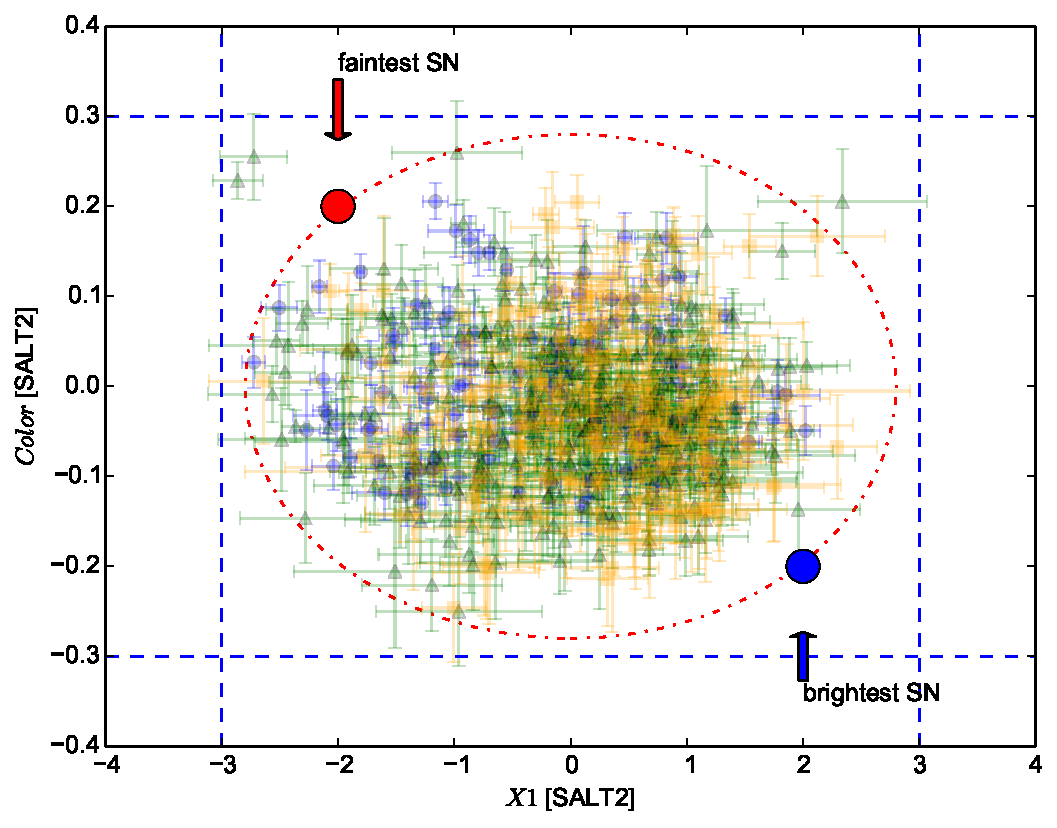
\includegraphics[width=0.75\linewidth]{sn_parameter_space.pdf}
\caption{JLA supernovae the $(X_1,Color)$ parameter space -- (blue:
  nearby, green: SDSS, orange: SNLS).  }
\label{fig:jla_X1_C}
\end{center}
\end{figure}

On the same figure, we have marked in red the faintest SN in that
parameter space ($X_1=-2, Color=0.25$). To be complete up to $z_{lim}$,
the survey has to deliver a cadence that allows to derive a luminosity
distance and a photometric identification for an event of such $X_1$
and Color, at a redshift $z_{lim}$.

\paragraph{Lightcurve quality requirements} Light curve quality
requirements have been discussed a few years ago, for the LSST-Euclid
paper \citep{2014A&A...572A..80A}. We summarize them below:

\begin{itemize}
\item the follow-up of each supernova must be good enough in the
  observer-frame bands that correspond to the $B$- and $V$-restframe
  spectrum ($3800 \angstrom < \lambda < 7000 \angstrom$).  At
  high-redshift, in particular, one should avoid relying on the $UV$
  restframe region to derive a distance, given the high intrinsic
  dispersion of SN~Ia at those wavelengths.
  
\item we require the light curve shape to be well sampled in the
  (restframe) phase interval $[-10;+30]$ days, with at least four
  visits before peak (each of those visits in any of the eligible
  band), and ten visits after peak.  To obtain this in the lower
  redshift region of the Hubble diagram, one requires an
  observer-frame cadence of 4 days.  In the upper redshift region (DDF
  fields), this requirement may be slightly relaxed. However, since we
  are going to rely exclusively on photometric identification, it is
  essential to secure a tight sampling of the SN color evolution at
  all redshift.
  
\item we require that the photon noise contribution to the distance
  measurement is subdominant w.r.t. the intrinsic dispersion of the
  SNe (after standardization).  There are several ways to quantify
  this.  With today's standardization techniques, the SN standardized
  distance modulus is:
  \begin{equation}
    \mu = m^\star_B + \alpha X_1 - \beta C - \cal{M}
  \end{equation}
  where $m^\star_B$ is the peak brightness in restframe $B$, $X_1$
  characterize the lightcurve width, and $C$ is an estimate of the
  restframe color $B-V$. $\alpha$, $\beta$ and $\cal{M}$ are global
  parameters, fit along with the cosmology. If the light curve is
  correctly sampled (see point above), the propagation of the
  measurement uncertainties affecting $m^\star_B$, $X_1$ and $C$ is
  dominated by the contribution of $\sigma_C$. Indeed, if the light
  curve is correctly sampled
  
  The dominant contribution is carried by the color (since
  $\beta \sim 3$). This means that requiring $\sigma C < 0.03$ ensures
  that $\sigma \mu < 0.1$, below the intrinsic dipersion in the Hubble
  diagram, after standardization.

\item each SN must have good quality measurements in at least three
  bands. We need two bands, covering the restframe $B$ and $V$ region,
  to constrain the restframe color of the SN. We need to provision an
  additional band (redder than restframe $V$), to enable next
  generation standardization techniques, that will likely rely on two
  restframe colors.
\end{itemize}


\paragraph{Conclusion} As a conclusion, evaluating the cadence boils
down to evaluating the follow-up of the faintest SN~Ia ($(X_1=-2,
C=0.25$) around $z = z_{lim}$. Our goal is to make sure that the light
curves of this SN of such events pass these requirements, throughout
the whole search season.

The requirements above fall into two categories: 
\begin{itemize}
\item we have  cadence requirements, which are easy  to evaluate (just
  count the number of visits before  and after peak in each band).  We
  require  a  restframe  cadence  of  3  days  or  better.   Following
  \cite{2014A&A...572A..80A}, we require an  observer frame cadence of
  4 days.

\item we also have depth requirements.  To quantify this, we can use
  the SNR on the SALT2 color, evaluated from the fit of the light
  curve of the faintest SN~Ia at different redshift and survey epochs:
  we require $\sigma_C < 0.03$ for all such SNe.

  An equivalent approach consists in placing requirements on the
  uncertainty of the amplitude of the light curve shape.  With three
  bands, we reach $\sigma_c < 0.03$ by requiring a SNR of 20 or better
  on the light curve amplitude, in each band separately.  It is
  somewhat simpler to evaluate, as it does not require to perform a LC
  fit (or fisher matrix estimate) with a SN LC model.
\end{itemize}

% Our goal is to make sure that the light curves of our faintest
% $(X_1=-2, C=0.25)$ SNe~Ia around $z = z_{lim}$ pass these requirements.


% ----------------------------------------------------------------------



\section{A metric to evaluate a cadence}
\label{sec:metric}

We now show how our LC requirements above translate into a simple
cadence-depth requirement.


\subsection{The signal-to-noise on the light-curve amplitude}

If we fit a model $A \times \ell(t)$ on a lightcurve $(t_i, y_i)$, the
least square estimate of the amplitude is:
\begin{equation}
  \hat{A} = \frac{\sum_i w_i \ell_i y_i}{\sum_i w_i \ell^2_i}
\end{equation}
where we note $\ell(t_i) = \ell_i$, and $w_i = 1 / \sigma_i^2$ the
measurement weights. The variance of $\hat{A}$ is:
\begin{equation}
  \mathrm{Var}(\hat{A}) = \left(\sum_i w_i \ell^2_i\right)^{-1}
\end{equation}
and signal to noise we get on the amplitude $\hat{A} /
\sigma_{\hat{A}}$ is:
\begin{equation}
  SNR = \left(\sum_i w_i L^2_i\right)^{1/2}
\end{equation}
where $L_i = A \times \ell_i$.  The weights can be expressed as a
function of the 5-$\sigma$ limiting flux of each visit $i$, $f_{i|5}$:
\begin{equation}
  SNR = 5 \times \left(\sum_i L^2_i f^{-2}_{i|5}\right)^{1/2}
  \label{eqn:snr}
\end{equation}
This metrics is easy to compute, all it takes is a tabulated model of
the light curve shape, and a cadence file, containing, for each visit,
an assessment of the $5\sigma$-depth reached during that visit. 


\subsection{Requirements on the survey cadence and depth}

Using the metric above, we can characterize the survey cadence and
depth that allow to fulfill the requirements above.

Let's define $\delta(t_i) = \delta_i$, which is equal to the number of
observations in an interval $\Delta t$ around $t_i$ (we express
$\delta_i$ in day$^{-1}$). The metric above can be rewritten:
\begin{equation}
  SNR = 5 \times \left(\sum_i \delta_i L^2_i f^{-2}_{i|5} \Delta t\right)^{1/2}
\end{equation}
where the sum runs on all the $\Delta t$ bins, in a observer frame
time interval covering the supernova lightcurve evolution. 

Let's define $f_{|5}$, the average 5-$\sigma$ limiting flux per visit,
in the band under consideration. The requirement above can be
rewritten:
\begin{equation}
  f_{|5} \left<\delta_i\right>^{-1/2} \leq \frac{5 \sqrt{\Delta t} \sqrt{\sum_i L_i^2}}{SNR}
  \label{eqn:global_metric}
\end{equation}
where $\left<\delta_i\right>$ is the cadence, weighted by the light
curve shape squared: $\left<\delta_i\right> = \sum_i \delta_i
L_i^2/\sum_i L_i^2$.  This sets a limit (in $\frac{e^-}{s}
\sqrt{day}$) on the product of the limiting flux times inverse square
root of the cadence.

This simple metric allows one to estimate the power of a cadence
without having to generate and fit supernova light curves.  Of course,
a supernova scientist is still needed, to compute the numerical values
of the upper limits that appears in equation \ref{eqn:global_metric}
For the records, we report these values in table
\ref{tab:cadence_depth_limit}. They have been computed with SALT-2.4
and the \code{SMTN-002} instrument model (see below).

\begin{table}[t]
\begin{center}
\caption{cadence-depth limit for a $[X_1=-2, C=0.25]$ SN~Ia and a target SNR=20/band}
\label{tab:cadence_depth_limit}
\begin{tabular}{l|rrrrr}
\hline
\hline
    $z$   &      $g$         &       $r$         &     $i$           &      $z$        &      $y$           \\
          &      \multicolumn{5}{c}{$[\mathrm{e^-/s \times \sqrt{day}}]$} \\
\hline
     0.2  &     386 &     526 &     470 &     251 &     103   \\
     0.3  &     123 &     207 &     193 &     150 &      52   \\
     0.4  &      39 &     110 &     109 &      84 &      33   \\
     0.5  &      15 &      64 &      59 &      51 &      27   \\
     0.6  &         &      35 &      38 &      36 &      17   \\
     0.7  &         &      18 &      28 &      23 &      13   \\
     0.8  &         &         &      21 &      16 &      10   \\
     0.9  &         &         &      14 &      13 &       7   \\
     1.0  &         &         &       9 &      10 &       5   \\
     1.1  &         &         &       5 &       8 &       4   \\
 
     % 0.2  &     916 &    1330 &    1262 &     704 &     289   \\
     % 0.3  &     284 &     513 &     495 &     421 &     149   \\
     % 0.4  &      86 &     267 &     279 &     224 &      91   \\
     % 0.5  &      31 &     153 &     148 &     131 &      76   \\
     % 0.6  &      12 &      81 &      94 &      92 &      43   \\
     % 0.7  &         &      42 &      69 &      57 &      34   \\
     % 0.8  &         &      17 &      52 &      39 &      25   \\
     % 0.9  &         &      11 &      32 &      31 &      17   \\
     % 1.0  &         &         &      20 &      26 &      12   \\
     % 1.1  &         &         &      11 &      20 &      11   \\
\hline
\end{tabular}
\end{center}
\end{table}

In the next sections, we show how the most recent \code{Minion\_1016}
cadence compares to our cadence-depth requirements, using the metric
above.  Before we do that, we must discuss the estimation of the
5-$\sigma$ depth. 


% ----------------------------------------------------------------------
\section{Instruments models \& Observing conditions}
\label{sec:instrument_model_summary}

Several models of the LSST throughput have been pusblished.  The
forecasts published in \cite{2014A&A...572A..80A} used the model
described in \cite[][hereafter LSE-40]{LSE-40}. 

\code{LSE-40} has been revised recently. The most recent model (as far
as we know) is presented in \cite[][hereafter SMTN-002)]{SMTN-002}.
The details and \code{LSE-40} and \code{SMTN-002} are discussed in
appendix \ref{sec:lsst_instrument_models}.  In particular, the model
characteristics are listed in tables \ref{tab:lse40} and
\ref{tab:smtn002}, the model throughputs are compared on figure
\ref{fig:throughput_comparison}.

We note that the throughput of \code{SMTN-002} is almost 40\% lower
than that of \code{LSE-40}.  While the latter model was probably a
little optimistic, \code{SMTN-002} seems a bit pessimistic for an
imager.  We have not been able to find, in the LSST literature, a
discussion on the differences between \code{SMTN-002} and
\code{LSE-40}.  Since the instrument throughput is an essential
ingredient of the survey depth, it is important to understand whether
\code{SMTN-002} was built as a realistic model, or as some kind of a
worst case assessment (as of today, we do not know).

On tables \ref{tab:lse40} and \ref{tab:smtn002} of appendix
\ref{sec:lsst_instrument_models}, we have reported the observing
conditions (median seeing and dark sky background) expected by in the
\code{LSE-40} and \code{SMTN-002} references.  They differ
significantly, \code{SMTN-002} being again more pessimistic than
\code{LSE-40}.

\code{Minion\_1016} uses \code{SMTN-002} (or a very similar instrument
model), but predicts larger median seeing values.  The median sky
obtained from the \code{Minion\_1016} logs is (expectedly) brigher
than the dark sky levels of \code{LSE-40} and \code{SMTN-002}. In the
$z$ band, the Minion sky levels are high, compared to what is measured
by DES.  In the $y$-band, the Minion prediction is strictly equal to
17.3 and shows no variation with the moon phase.  We believe that the
\code{Minion\_1016} sky level is not valid in the $y$-band. As we will
see in the following of this note, this affects our ability to predict
the effective depth of the DDF survey.

\begin{figure}[t]
\begin{center}
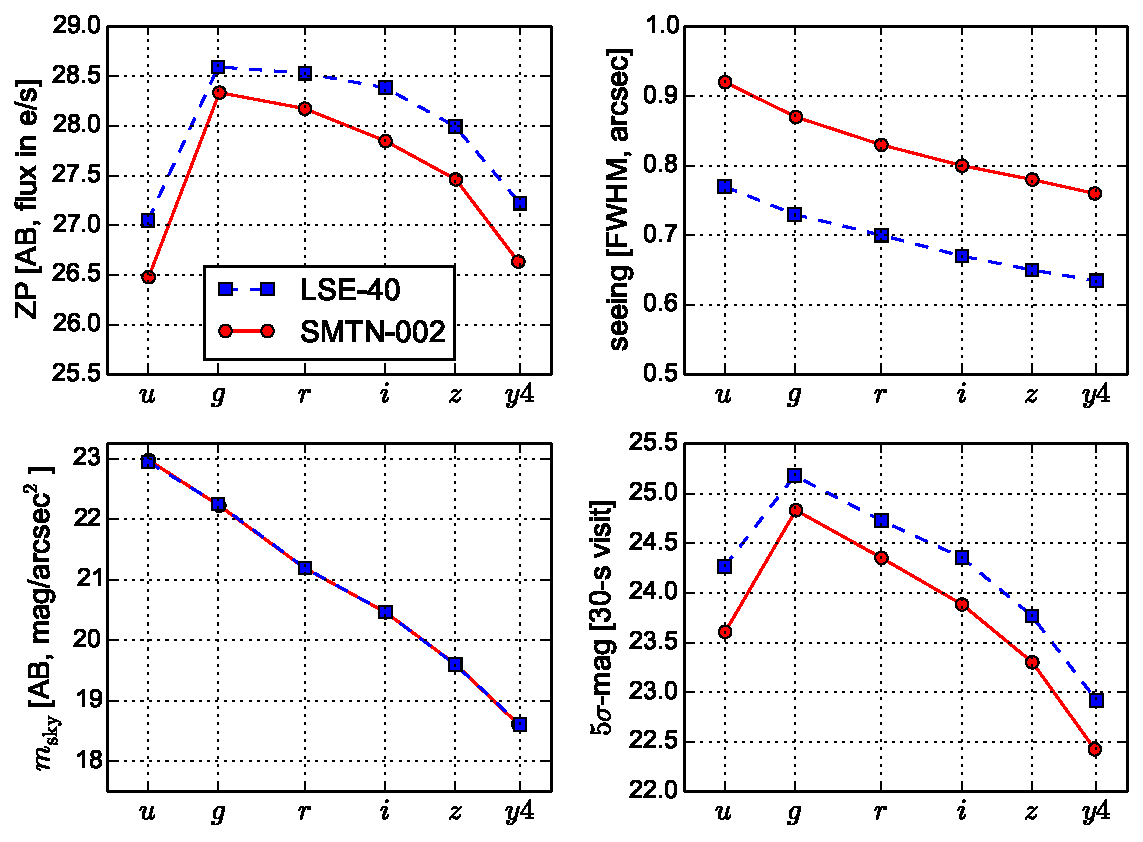
\includegraphics[width=\linewidth]{lsst_model_summary.pdf}
\caption{Zero-points, median seeing, dark sky mags and limiting mags}
\label{fig:lsst_model_summary}
\end{center}
\end{figure}

% We have compared all those values with the median seeing and sky
% background computed from the \code{Minion\_1016} logs. Again, the
% median seeing of Minion is considerably worse than that of
% \code{SMTN-002}.  The median sky of Minion is also significantly
% brighter (but here, we are comparing a median sky background with the
% assessment of a dark sky background).

On figure \ref{fig:lsst_model_summary}, we compare the throughtput
(ZP), median seeing and sky of LSE-40, SMTN-002 and
\code{Minion\_1016}.  On the lower left panel, we estimate the typical
5-$\sigma$ depth of a 30-second LSST visit, from (1) the \code{LSE-40}
and \code{SMTN-002} instrument model and observing conditions, and (2)
the \code{SMTN-002} instrument model and Minion median observing
conditions. We note that the median depth predicted by \code{Minion}
is 0.8 to 1 mag lower that what was inferred from LSE-40 in the
\cite{2014A&A...572A..80A} study.


As a conclusion, the results presented below will need to be updated
as our understanding of the instrument model and observing conditions
at Cerro Pachon improves.




% ----------------------------------------------------------------------
\section{The deep SN survey on the DDF fields}
\label{sec:ddf_cadence}


\subsection{Nominal cadence}

Before we evaluate the \code{Minion\_1016} cadence, let's assess the
quality of the SN follow-up if the survey delivers a nominal 4-day
cadence. We adopt the sky brightness values and median seeing values
that are reported in \cite{LSE-40} and \cite{SMTN-002} respectively.

\begin{figure*}
\begin{center}
\subfigure[\code{SMTN-002} -- 600-s visits]{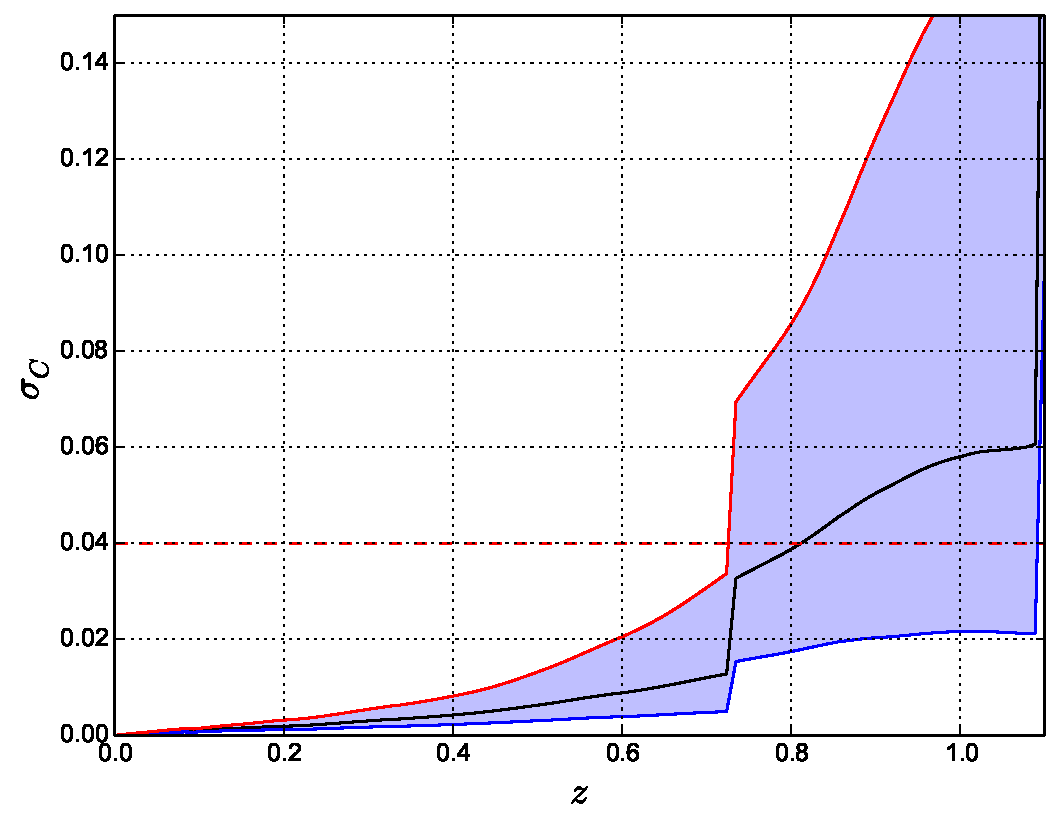
\includegraphics[width=0.49\linewidth]{sigc_lsstpg_ddf_600.pdf}}
\subfigure[\code{SMTN-002} -- 1800-s DDF visits]{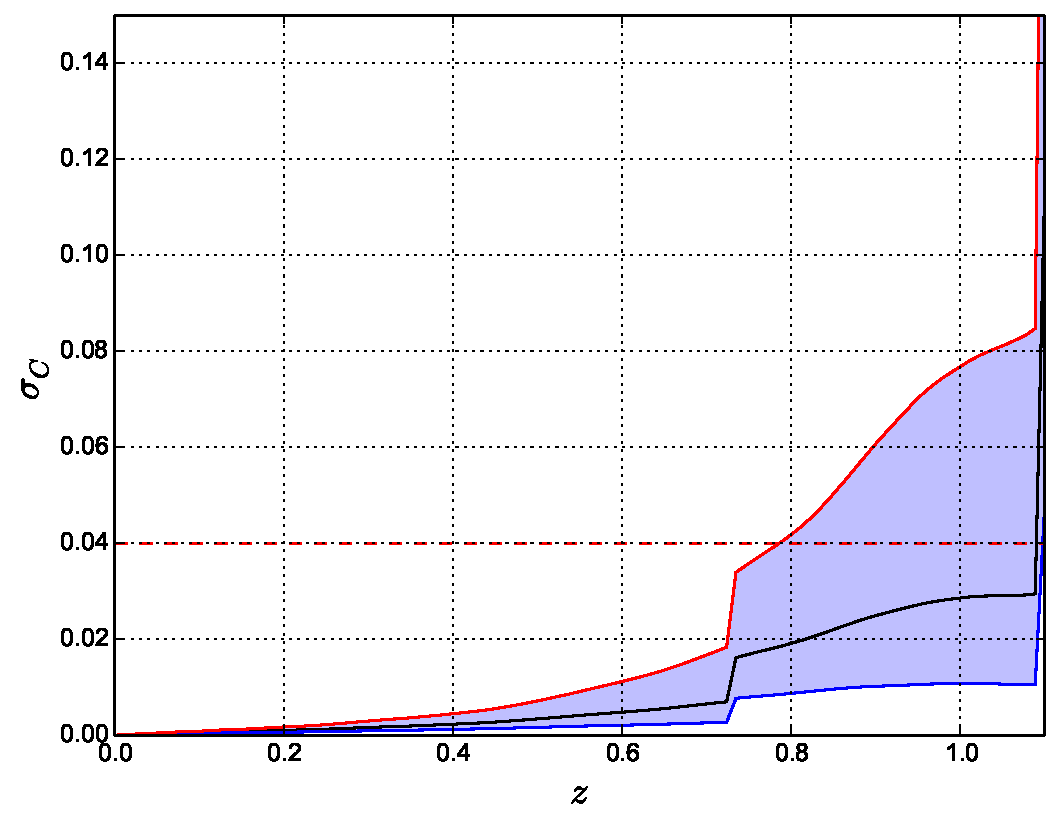
\includegraphics[width=0.49\linewidth]{sigc_lsstpg_ddf_1800_cad3.pdf}}
\subfigure[\code{SMTN-002} -- 600-s visits]{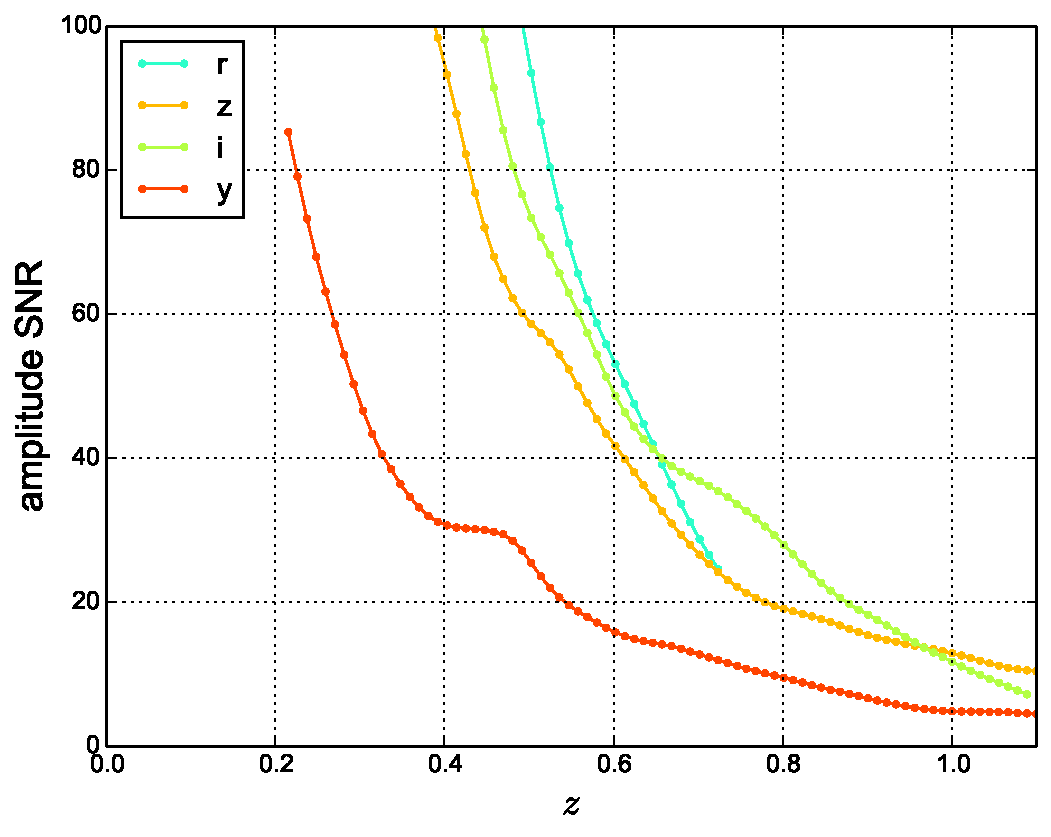
\includegraphics[width=0.49\linewidth]{snr_lsstpg_ddf_600.pdf}}
\subfigure[\code{SMTN-002} -- 1800-s DDF visits]{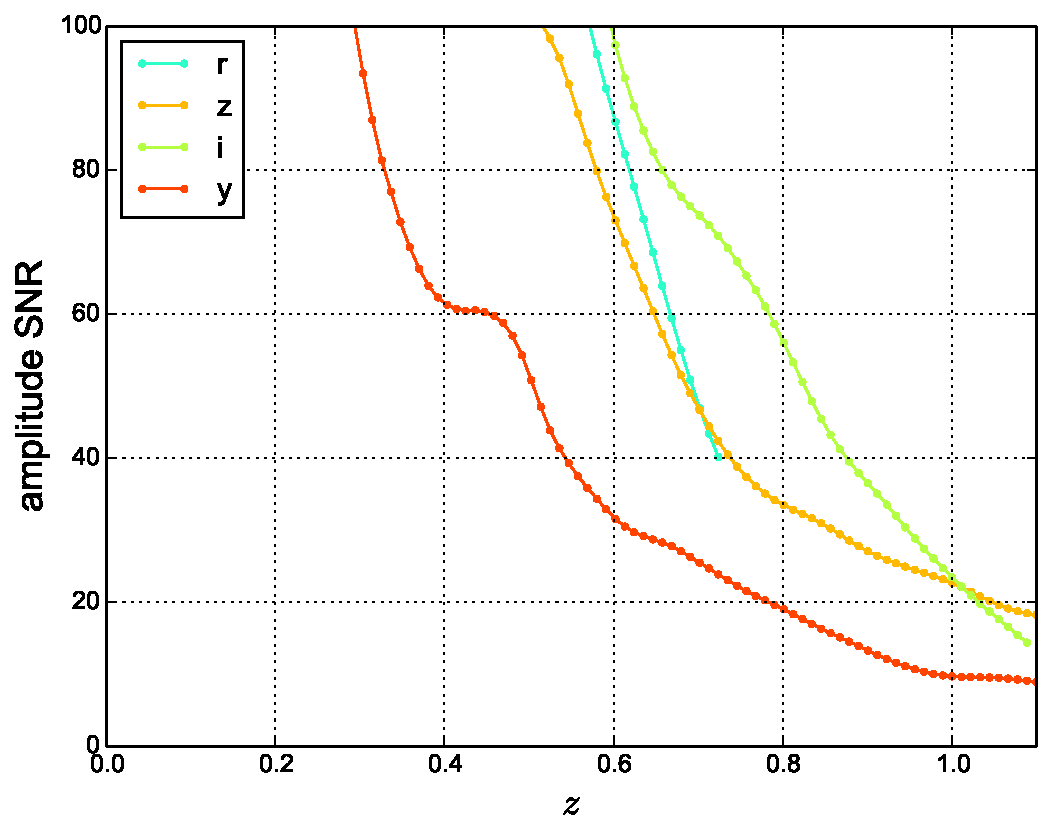
\includegraphics[width=0.49\linewidth]{snr_lsstpg_ddf_1800_cad3.pdf}}
\end{center}
\caption{Upper panels: $\sigma_C$ (shot noise only) obtained on the
  DDF fields as a function of redshift.  On the left, for the standard
  (r: 600-s, i: 600-s, z: 780-s, y: 600-s) visits and a 4 day cadence,
  on the right for 1200-s visits (same cadence). Lower panels: SNR
  obtained on the light curve amplitude, as a function of
  redshift. Left and right: same observing conditions.}
\label{fig:sigc_vs_z_4_day_cadence}
\end{figure*}

The quality of the distances is a function of the resolution we get on
the SN color.  On figures \ref{fig:sigc_vs_z_4_day_cadence} and
\ref{fig:sigc_vs_z_2_day_cadence} we display how $\sigma_C$ varies
with redshift, for the mean SN (black curve), and our faint and bright
fiducial SNe (red and blue curves respectively).  We present 4
different scenarios:
\begin{description}
\item[Figure \ref{fig:sigc_vs_z_4_day_cadence}, left panels] standard
  DDF visits (r: 600-s, i: 600-s, z: 780-s, y: 600-s); 4-day cadence;
  instrument model and observing conditions taken from
  \code{SMTN-002}.
\item[Figure \ref{fig:sigc_vs_z_4_day_cadence}, right panels]
  increasing the visits to 1200-s ($rizy$); 4-day cadence; instrument
  model and observing conditions taken from \code{SMTN-002}.]
\item[Figure \ref{fig:sigc_vs_z_2_day_cadence}, left panels] 1200-s in
  ($rizy$), but with a 2-day cadence; instrument model and observing
  conditions taken from \code{SMTN-002}.]
\item[Figure \ref{fig:sigc_vs_z_2_day_cadence}, left panels] 1200-s in
  ($rizy$); 2-day cadence; instrument model and observing conditions
  taken from \code{LSE-40}.]
\end{description}

The sharp increase of $\sigma_C$ around $z \sim 0.7$ corresponds to
when the $r$-band starts sampling the $\lambda < 3600\AA$ region. As
discussed above, SNe are much more variable in the UV, hence we cannot
rely on this spectral region to derive distances (until somebody
figures out how to standardize SNe in the UV).

The bottom panel shows the SNR on the amplitude of the lightcurves for
our faint fiducial SN. We see that we are fine, as long as we can
secure a SNR of 20 in each band buyt $y$. In $y$, obtaining this level
of signal to noise seems to be very hard. Obtaining $SNR=10$ up to
$z\sim 0.8$ does the job, as long as the two other bands reach a SNR of 20. 


\begin{figure*}
\begin{center}
\subfigure[\code{LSE-40} -- 600-s -- 4 day cadence]{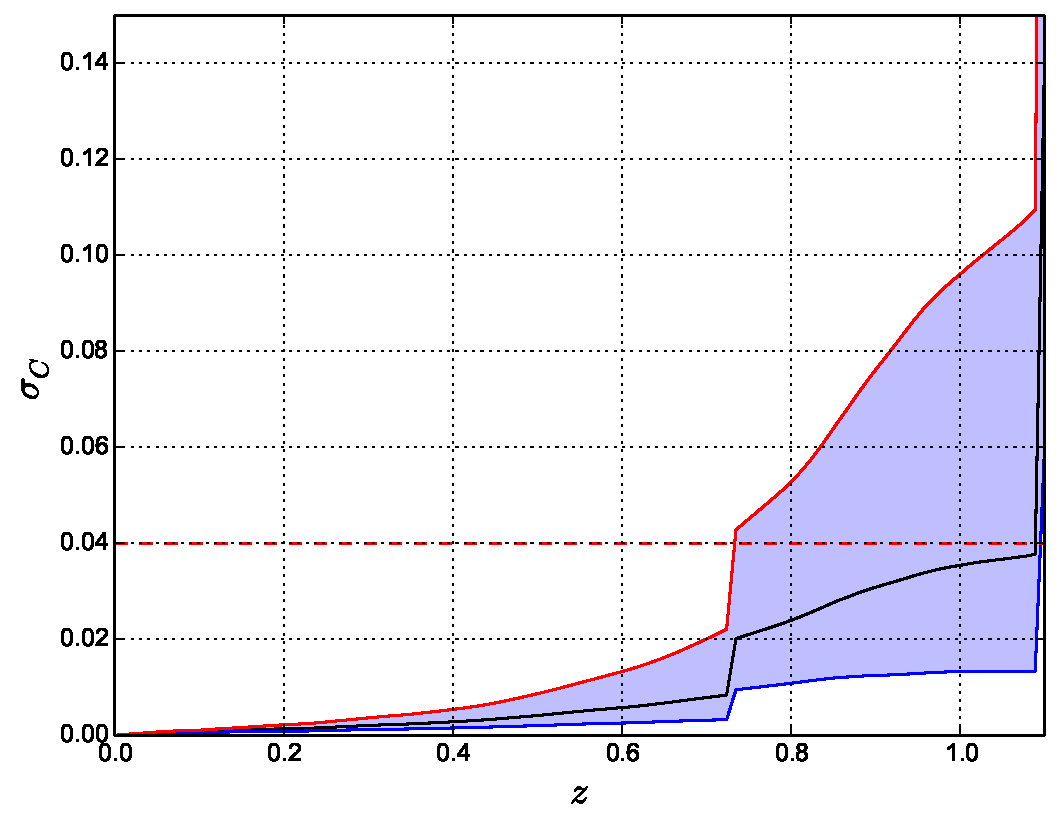
\includegraphics[width=0.49\linewidth]{sigc_lsst_ddf_600.pdf}}
\subfigure[\code{LSE-40} -- 1800-s -- 3 day cadence]{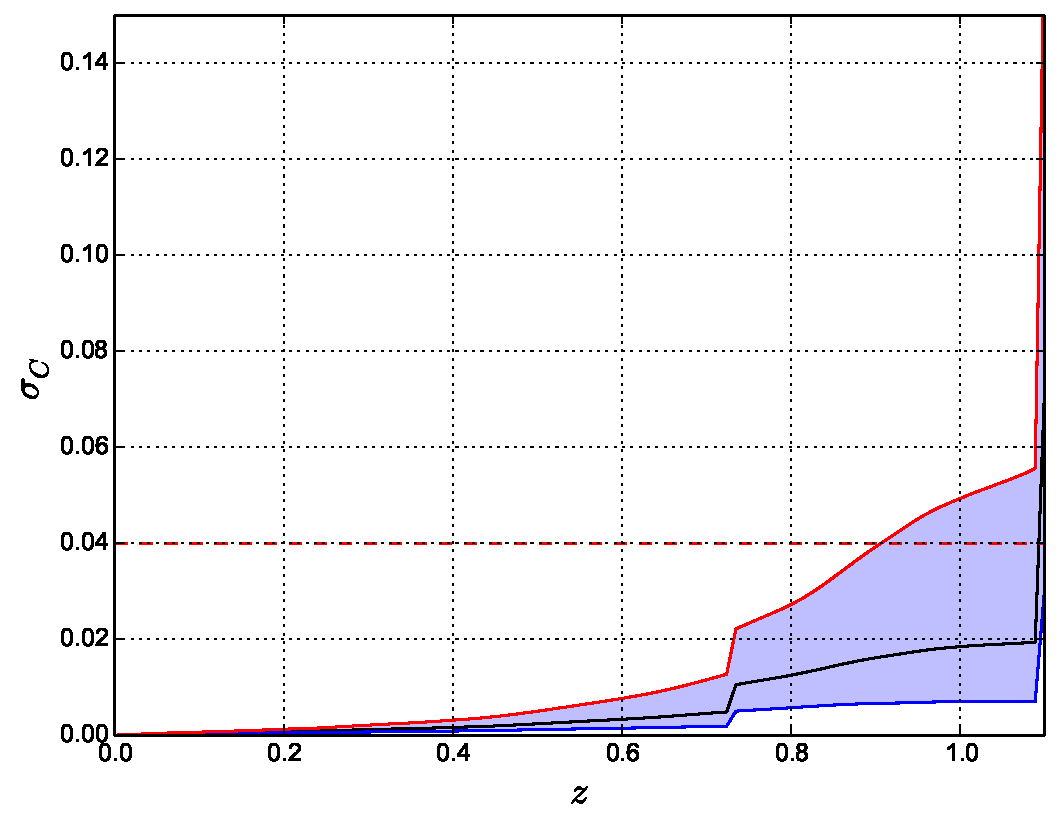
\includegraphics[width=0.49\linewidth]{sigc_lsst_ddf_1800_cad3.pdf}}
\subfigure[\code{LSE-40} -- 600-s -- 4 day cadence]{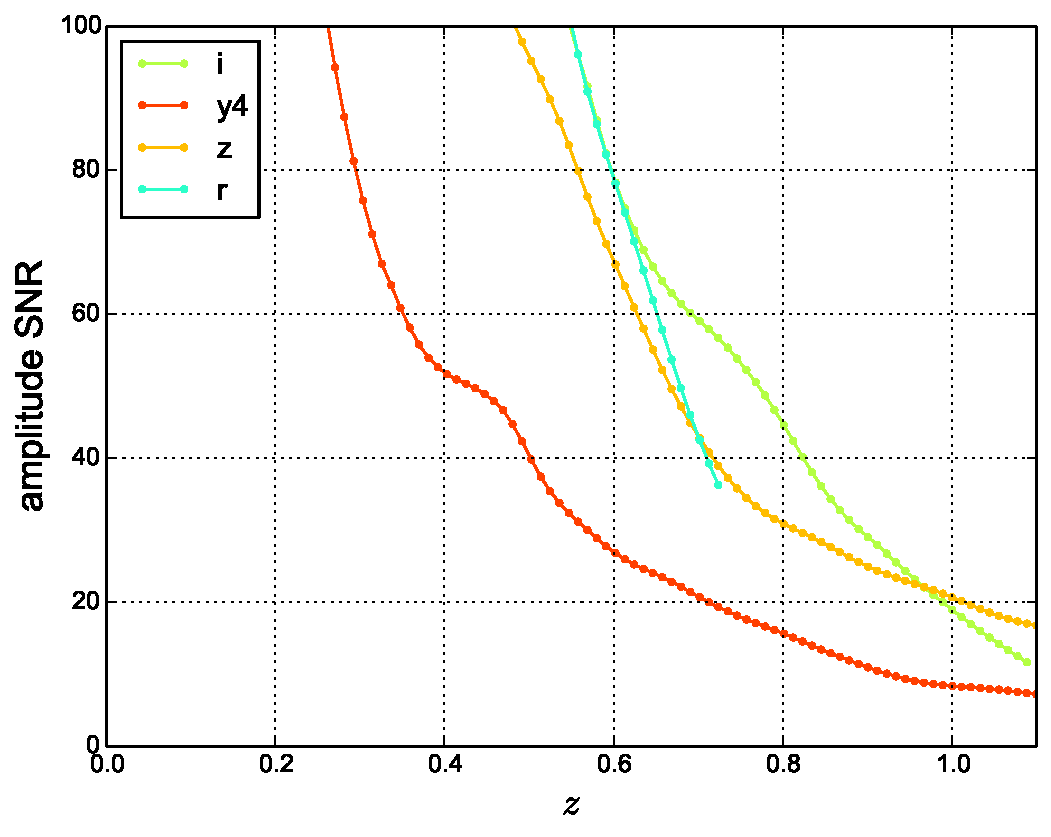
\includegraphics[width=0.49\linewidth]{snr_lsst_ddf_600.pdf}}
\subfigure[\code{LSE-40} -- 1800-s -- 3 day cadence]{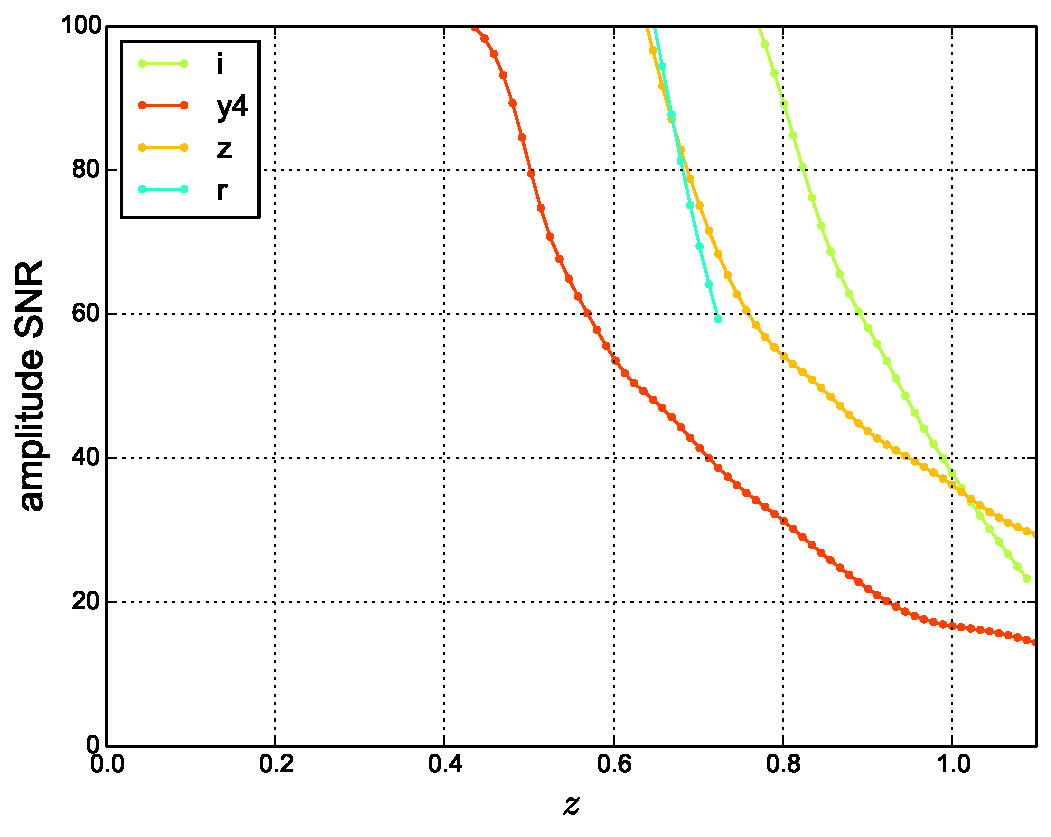
\includegraphics[width=0.49\linewidth]{snr_lsst_ddf_1800_cad3.pdf}}
\end{center}
\caption{Same as figure \ref{fig:sigc_vs_z_4_day_cadence} with a 2-day
  cadence.  Left column: \code{SMTN-002}.  Right column:
  \code{LSE-40}.  Doubling the cadence and the exposure time,
  allows-one to build a sample that is complete up to $z \sim 0.75$ if
  we assume that \code{SMTN-002} is a correct representation of the
  instrument performances and 0.9 if we believe the official
  \code{LSE-40} requirements.}
\label{fig:sigc_vs_z_2_day_cadence}
\end{figure*}

These figures are a representative subset of what has been explored.
We see that obtaining a good follow-up for the faint end of the SN
distribution requires at least doubling the exposure time of each
visit {\em and} the cadence. Doing so (and assuming \code{SMTN-002})
allows one to build a sample that is almost complete up to $z \sim
0.8$. In the following of this section, we will adopt this as our
nominal scenario. Table \ref{tab:nominal_scenario_DDF} summarizes the
cadence, exspoure times and the average $5-\sigma$ depth per visit.

\begin{table*}
\begin{center}
\caption{A nominal scenario for the DDF that allows to build a SN
  sample complete up to $z \sim 0.75$.}
\label{tab:nominal_scenario_DDF}
\begin{tabular}{l|cccc}
\hline
\hline
              & $r$ & $i$ & $z$ & $y$ \\
\hline 
$T_{exp}$      & 1200 & 1800 & 1800 & 1800 \\
$m_{5\sigma}$  & 26.43    & 26.16    &  25.56    &  24.68   \\
cadence       &  \multicolumn{4}{c}{3 days} \\
Target amplitude SNR & $>25$ & $>60$ & $>35$ & $>20$ \\
\hline
\end{tabular}
\end{center}
\end{table*}

Finally, we note, from figure \ref{fig:sigc_vs_z_2_day_cadence} the
impact of changing the instrument model on the effective depth of the
survey: with the same time budget, we increase very sizeably the depth
of the survey (from $z \sim 0.75$ to almost $z\sim 0.9$), with a
significant increase of the quality of the average lightcurve.  We
think it is essential for the SNWG members to understand the origin of
the differences between \cite{LSE-40} and \cite{SMTN-002}.


\subsection{The DDF cadence from \code{Minion\_1016}}
\label{sec:results}


\begin{figure*}[t]
\begin{center}
\subfigure[$r$]{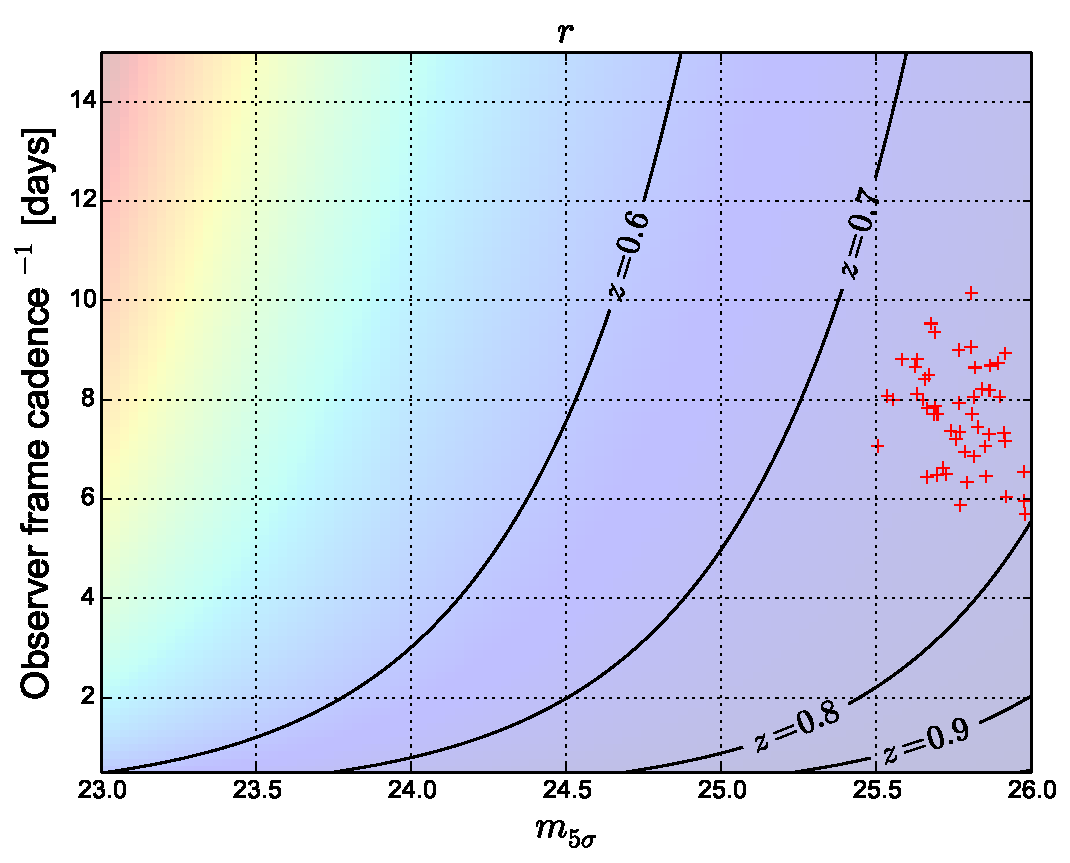
\includegraphics[width=0.48\linewidth]{m5_cadence_limits_r.pdf}}
\subfigure[$i$]{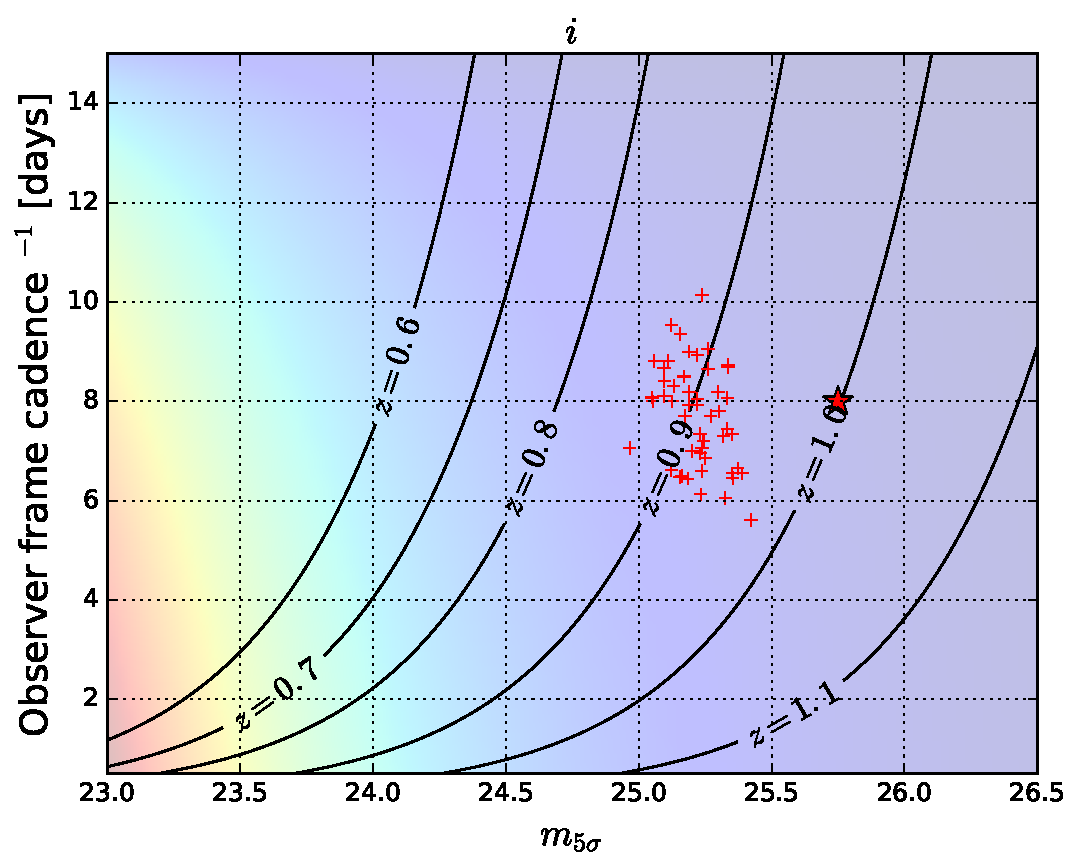
\includegraphics[width=0.48\linewidth]{m5_cadence_limits_i.pdf}}\\
\subfigure[$z$]{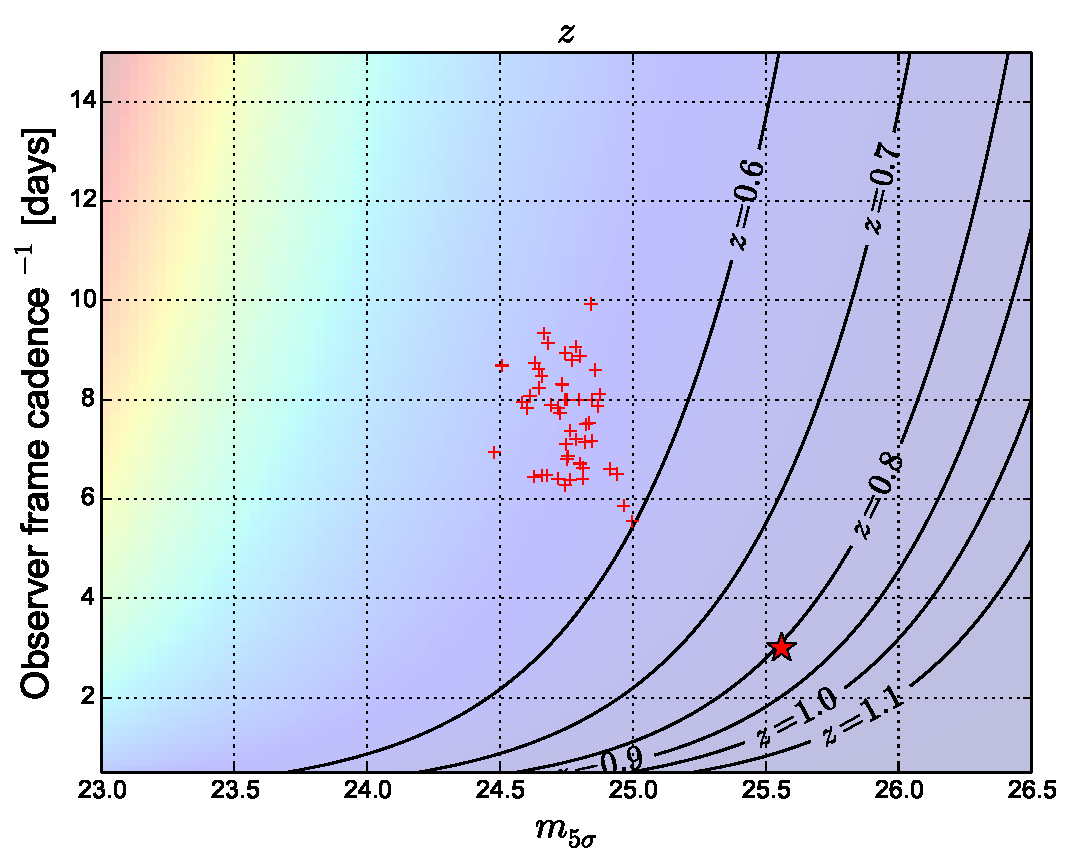
\includegraphics[width=0.48\linewidth]{m5_cadence_limits_z.pdf}}
\subfigure[$y$]{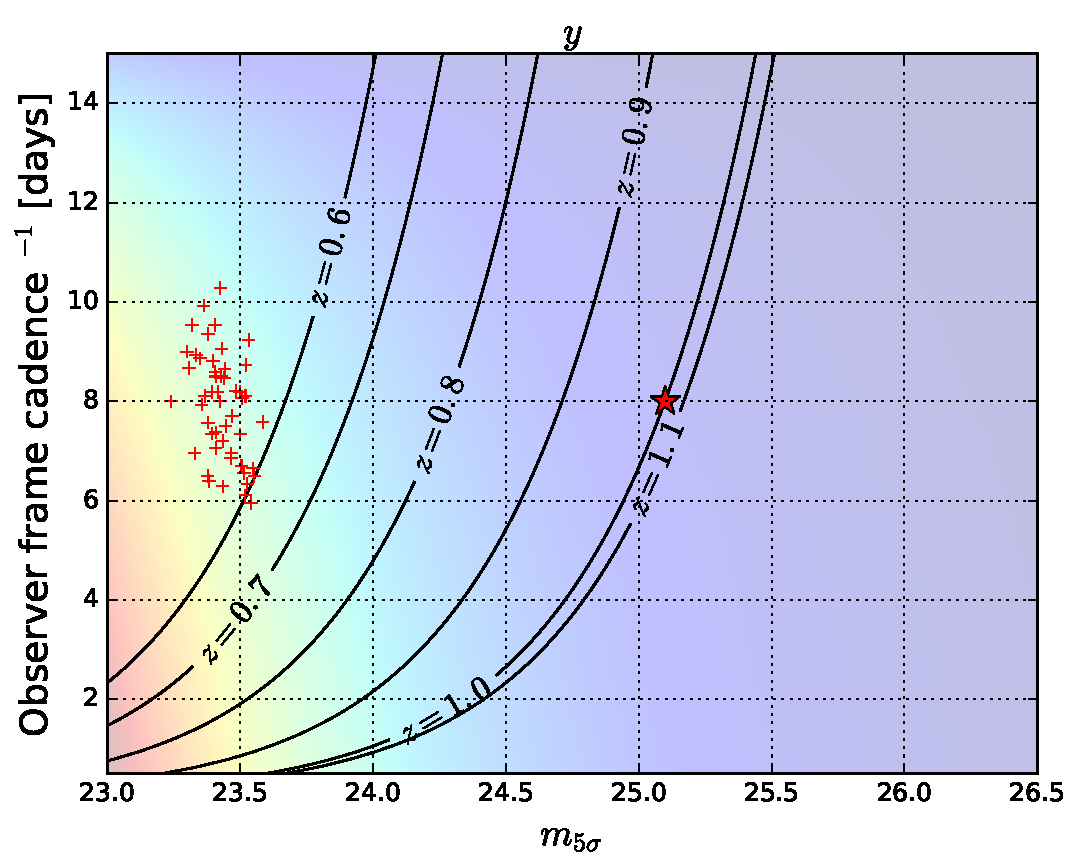
\includegraphics[width=0.48\linewidth]{m5_cadence_limits_y.pdf}}
\caption{The cadence {\em vs.} depth requirements for the DDF LSST SN
  survey in the $r,i,z$ and $y$-bands. The color scale corresponds to
  the metric described in equation \ref{eqn:global_metric}.  The lines are
  the contour-levels computed for the limits indicated on table
  \ref{tab:cadence_depth_limit}. To fulfill the SNR requirements at a
  given redshift, one has to be {\em below} the corresponding
  line. The stars indicate an ambitious -- but attainable -- goal for
  a DDF survey.  The red crosses show what the survey can currently
  deliver according to \code{Minion\_1016}. }
\label{fig:m5_cadence_limits_ddf}
\end{center}
\end{figure*}

\paragraph{Median depth and cadence needed to match the requirements}
The constrains described in equation \ref{eqn:global_metric} can be
represented graphically in the $m_{5\sigma}$-cadence plane. We do this
on figure \ref{fig:m5_cadence_limits_ddf}, for the bands of interest
for an intermediate and/or deep survey ($rizy$).

This plot allows one to quantify the nominal survey cadence and depth
that are required to operate a survey up to a given redshift limit.
As we target an observer-frame cadence ($^{-1}$) of 4 days, we need to
reach depths of 26.3, 25.7 and 25.7 per-visit, in the $i, z$ and $y$
bands, respectively. We may relax the cadence requirement, but this
needs to be compensated by increasing the median visit depth.

We summarize in table \ref{tab:depth_for_ddf} the depth that needs to
be reached, assuming a cadence of 4 observer-frame days. We also
report the exposure times that are required to reach such a depth,
assuming the median (Minion) observing conditions. 

\begin{table*}[t]
\begin{center}
  \caption{Target 5-$\sigma$ depth for each visit of the Deep
    SN-survey, assuming a 4 day cadence. Per-visit exposure times to
    reach these depth. }
\label{tab:depth_for_ddf}
\begin{tabular}{l|cccc}
\hline
\hline
                         & $r$ & $i$  & $z$  & $y$  \\
\hline
Target 5-$\sigma$ depth  & 25.8  & 26.3 & 25.7 & 25.6 \\
Default $T_{exp}$ [s]     &  600   & 600  & 780  & 600  \\
\hline
seeing [median, Minion]  &  0.98 & 0.92  & 0.83 &  0.86 \\
sky    [median, Minion]  & 20.9  & 19.9  & 19.1 &  17.3 \\
$T_{exp}$ [s]             &        & 5000  & 5000 & $> 10000$ \\
\hline
seeing [LSE-40]          & 0.70  & 0.67  & 0.65  &  0.63 \\
sky    [LSE-40]          & 21.2  & 20.5  & 19.6  & 18.6  \\
$T_{exp}$ [s]             & $<600$  & 1000  & 1000  &  3600 \\
\hline
seeing [SMTN-002]        & 0.83 & 0.80 & 0.78 &  0.76   \\
sky    [SMTN-002]        &  21.2 & 20.5  & 19.6 &  18.6 \\
$T_{exp}$ [s]             &  $<600$ &  2400  & 2400  &  $> 10000$     \\
\hline
\end{tabular}
\end{center}
\end{table*}





\paragraph{Where we are now, with \code{Minion\_1016}} We can show on
the same graph the median cadence and depth computed for each DDF
field, from the \code{Minion\_1016} sequences. We have 5 DDF, each
spanning 10 search seasons (ten years of operations).  This gives 50
cadence-depth realizations, which we represent with red crosses.

To match the cadence-depth requirements at a given redshift, we need
to be {\em below} the corresponding line {\em in the $i$, $z$ and $y$
  bands simultaneously}. We see that the average cadence delivered by
the survey is about a factor 2 below our target. In the $i$ and $z$
bands, the depth is adequate to obtain a survey complete up to $z \sim
0.8$, however, the predicted $y$-band depth is far below what is
needed.


\begin{figure*}[t]
  \begin{center}
    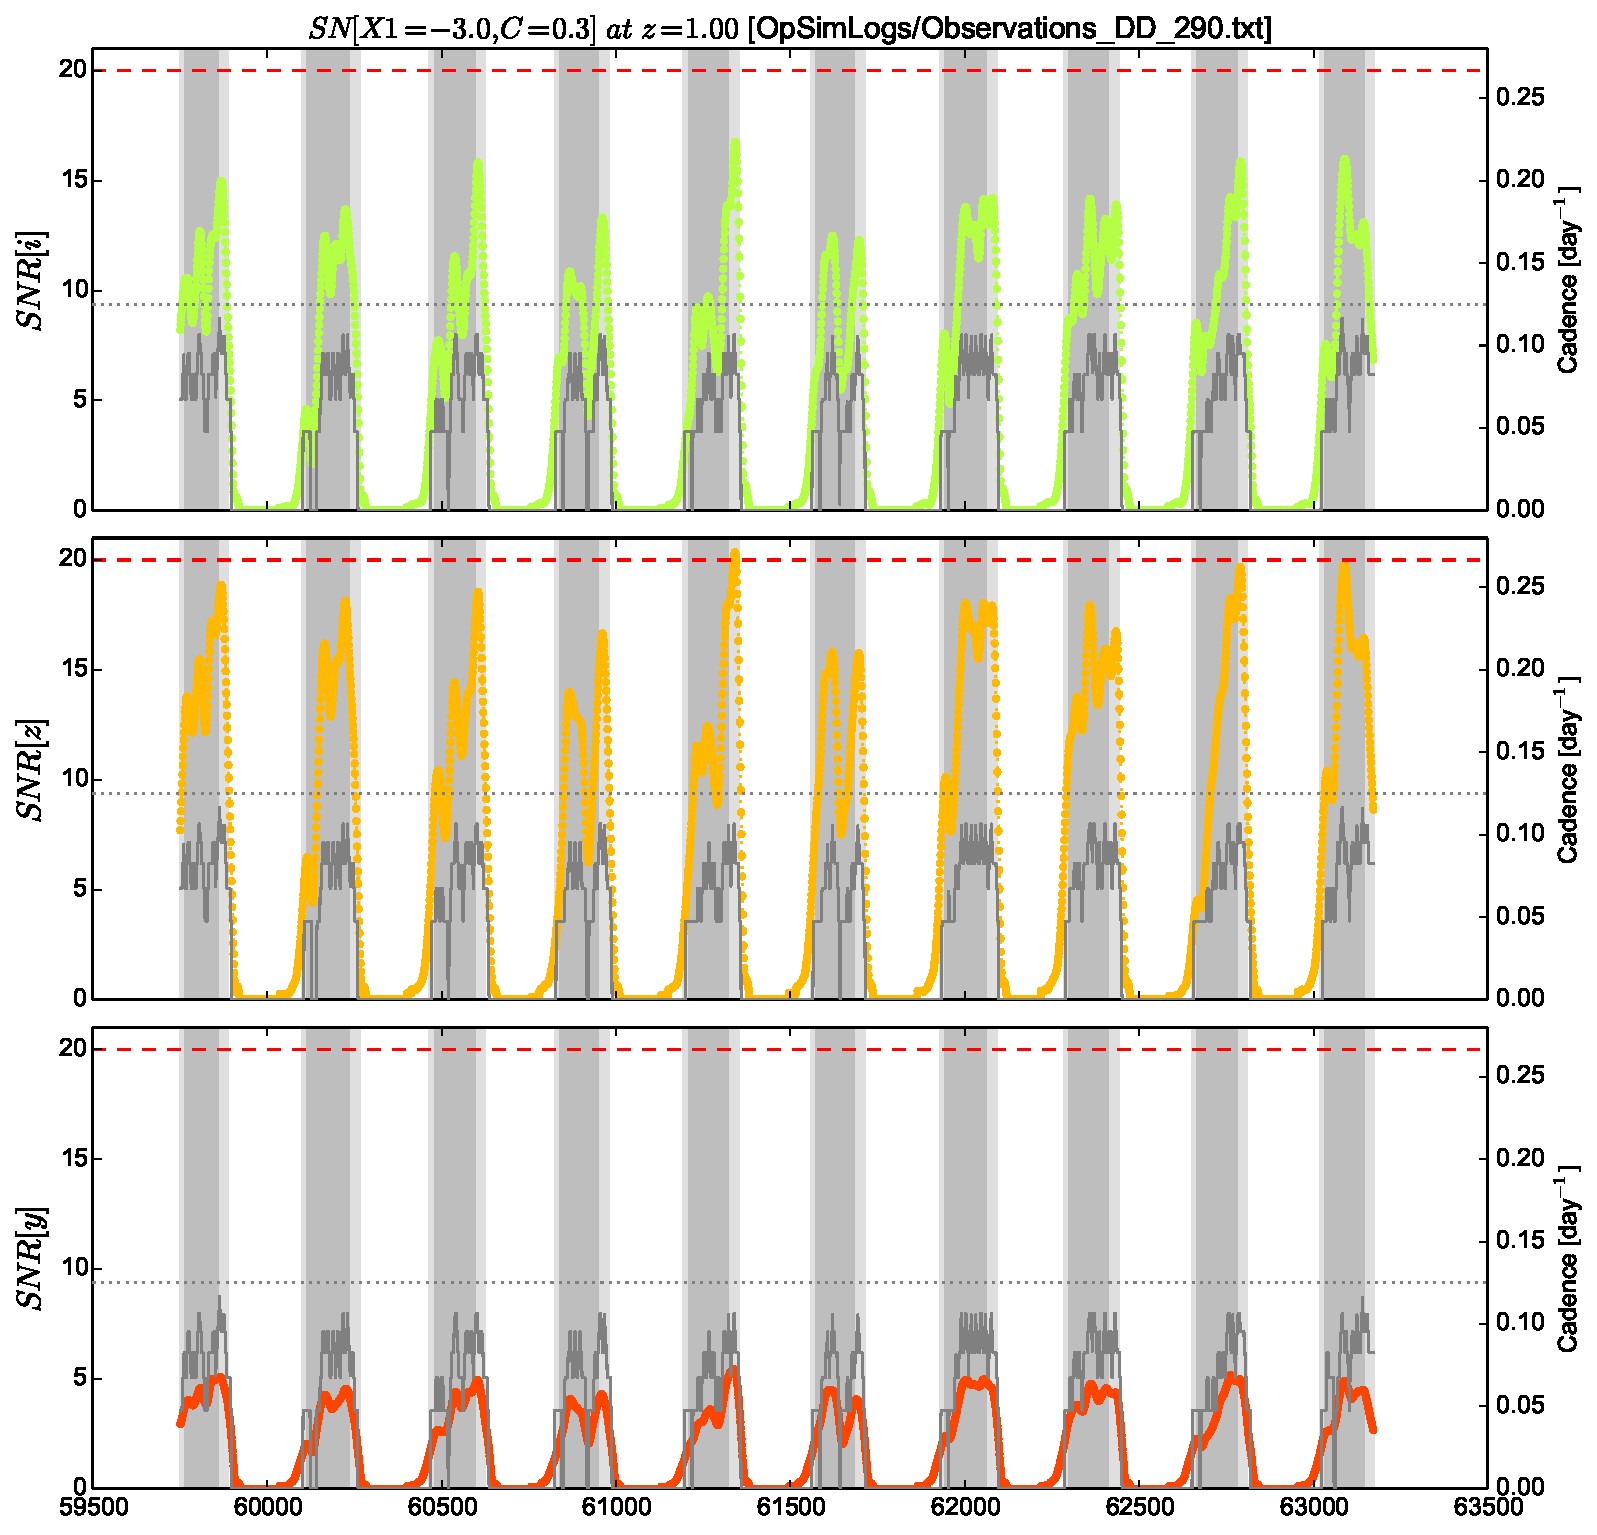
\includegraphics[width=\linewidth]{metric_DD_290.pdf}
    \caption{Colored lines: the SNR of the estimated amplitude of a
      $[X_1=-2, C=0.25]$ SN~Ia at a redshift $z = 1$ as a function of
      peak MJD, computed for the \code{Minion\_1016} cadence and depth
      for field \#290. The SNR target is shown with the dashed red
      line.  Thin gray lines: the cadence delivered in that band,
      averaged in 30-day a sliding window.  The cadence target is
      represented as a dotted line. The plot extends over the 10 years
      of survey operations. The gray area corresponds to the search
      seasons for that field. The light gray area corresponds to the
      margins for which the SN has no points before (resp after)
      peak.}
    \label{fig:snr_metric}
  \end{center}
\end{figure*}


\paragraph{SN specific metric} The global metric above is very
efficient to assess a nominal cadence and depth, and to evaluate a
whole OpSim run. We also want to check the regularity of the cadence
over a season. This can be done by computing, in each relevant band,
the SNR that can be obtained on the amplitude of the lightcurve
(following equation \ref{eqn:snr}), as a function of the SN peak date.

This is what we show  on figure \ref{fig:snr_metric}, for our fiducial
faint SN at a  redshift $z=1$, for one of the DDF  fields, and for the
whole duration of  the survey operations. As we can  see, we are below
our target SNR of  20 in all the relevant bands. We  also see that the
cadence and depth  is not constant over one single  season. We suggest
that adding  such a  metric in  the scheduler  would allow  to control
finely the depth of the survey  over the whole duration of the season.
The goal would  be to reach our target  SNR shortly\footnote{say, $-15
  \times (1  + z_{lim})$ observer-frame  days} after the  beginning of
the first observations of the season,  and to schedule the cadence and
depth of the visits in such a  way that the SNR stays above the target
SNR in all relevant bands during the season.


\paragraph{What is the effective depth of the DDF survey ?}

On figure \ref{fig:sigma_color_vs_z}, we show the SALT2 color
uncertainty (shot noise only) as a function of the redshift of our
$X_1=-2, C=0.25$ SN for the first season of field \#290 (the one of
figure \ref{fig:snr_metric}).  We see that the redshift limit is
$z_{lim} \sim 0.7$.  This is comparable to what SNLS was able to
deliver, and probably far below what LSST can deliver. 

\begin{figure}[t]
\begin{center}
\subfigure[season \#1]{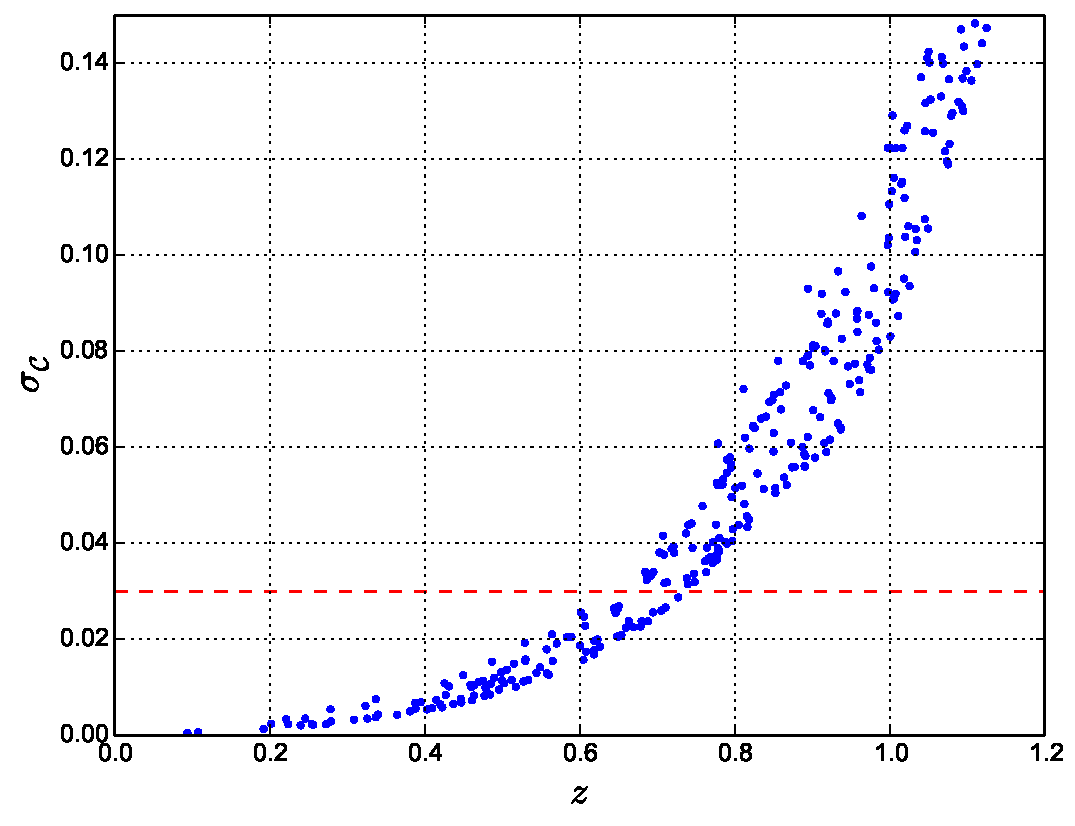
\includegraphics[width=0.48\linewidth]{sigma_c_vs_z_DDF_290_0.pdf}}
\subfigure[season \#3]{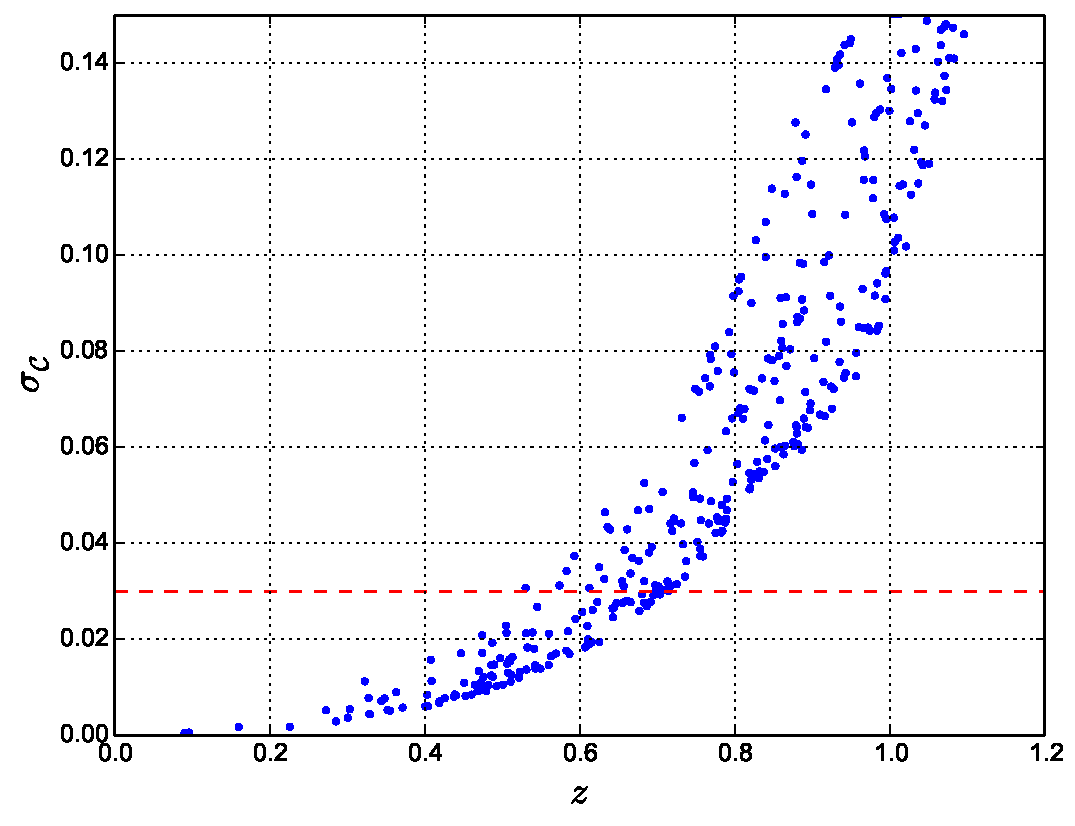
\includegraphics[width=0.48\linewidth]{sigma_c_vs_z_DDF_290_2.pdf}}
\caption{Color uncertainty (shot noise only) as a function of redshift, for two seasons of DDF field \#290.}
\label{fig:sigma_color_vs_z}
\end{center}
\end{figure}


\paragraph{~} Our (temporary) conclusions for the DDF fields are that:
\begin{itemize}
\item in all bands, the cadence is about a factor 2 lower than our target.
\item the season-to-season dispersion of the cadence is
  significant. It could be reduced if one monitors the recent cadence
  and depth within the scheduler, and tune the cadence and depth
  accordingly.
\item at the cadence delivered by \code{OpSim}, the $i$ and $z$ depth
  is 0.5-mag and 0.25-mag lower than our target (resp). In the
  $y$-band the depth is 1.75-mag below our target, but this is
  probably due to the fact that the Minion sky level is incorrect in that band.
\item in the $i$ and $z$ bands, increasing the cadence by a factor 2,
  and keeping the per-visit depth similar allows one to reach the
  target. In the $y$ band, we do not know (yet) what to say, except
  that we need to check the sky model.
\item the cadence and depth vary quite significantly as a function of
  time, within a season. Again, computing on the fly the amplitude SNR
  for the [$X_1=-2, C=0.25$] SN at the targeted limiting redshift, and
  making sure that it stays above 20 in the $izy$ bands, would allow
  to to stay above $z_{lim}$ for the whole duration of the search
  season.
\end{itemize}



% ----------------------------------------------------------------------
\section{The Wide LSST SN survey}
\label{sec:wide_cadence}

\subsection{Nominal cadence}

\begin{figure*}
\begin{center}
\subfigure[\code{SMTN-002} -- standard visits]{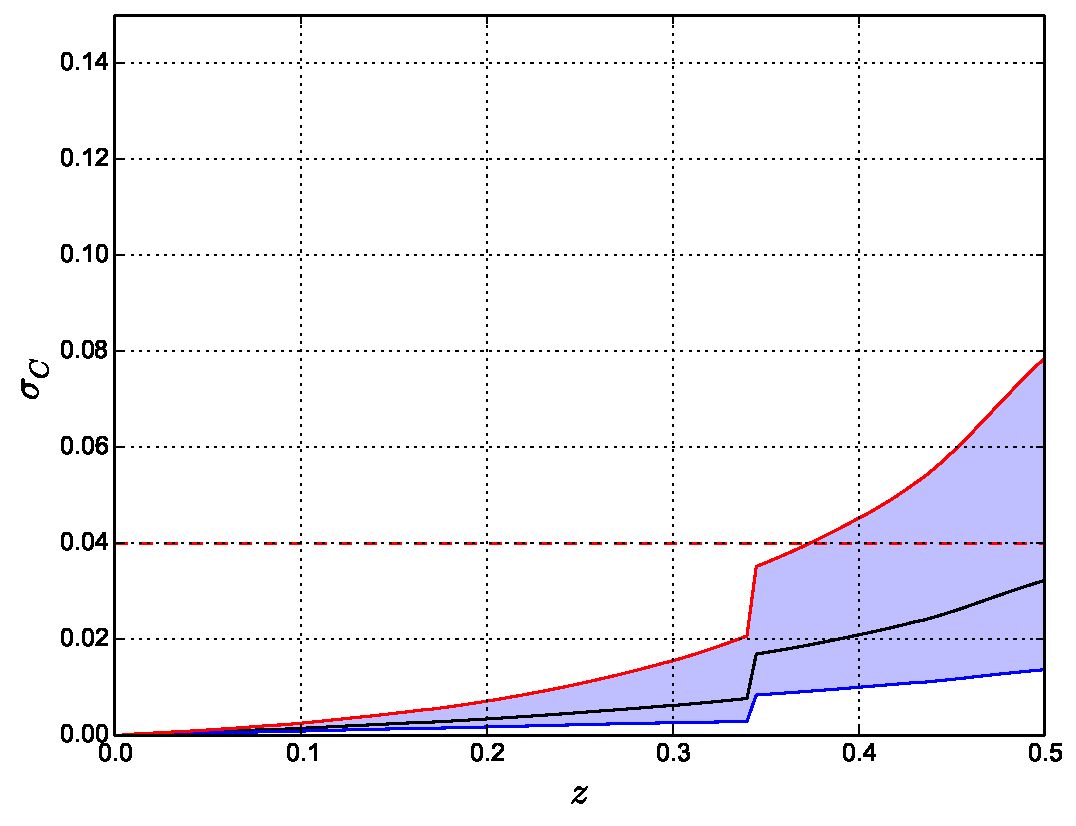
\includegraphics[width=0.49\linewidth]{sigc_lsstpg_wide_30.pdf}}
\subfigure[\code{SMTN-002} -- deeper]{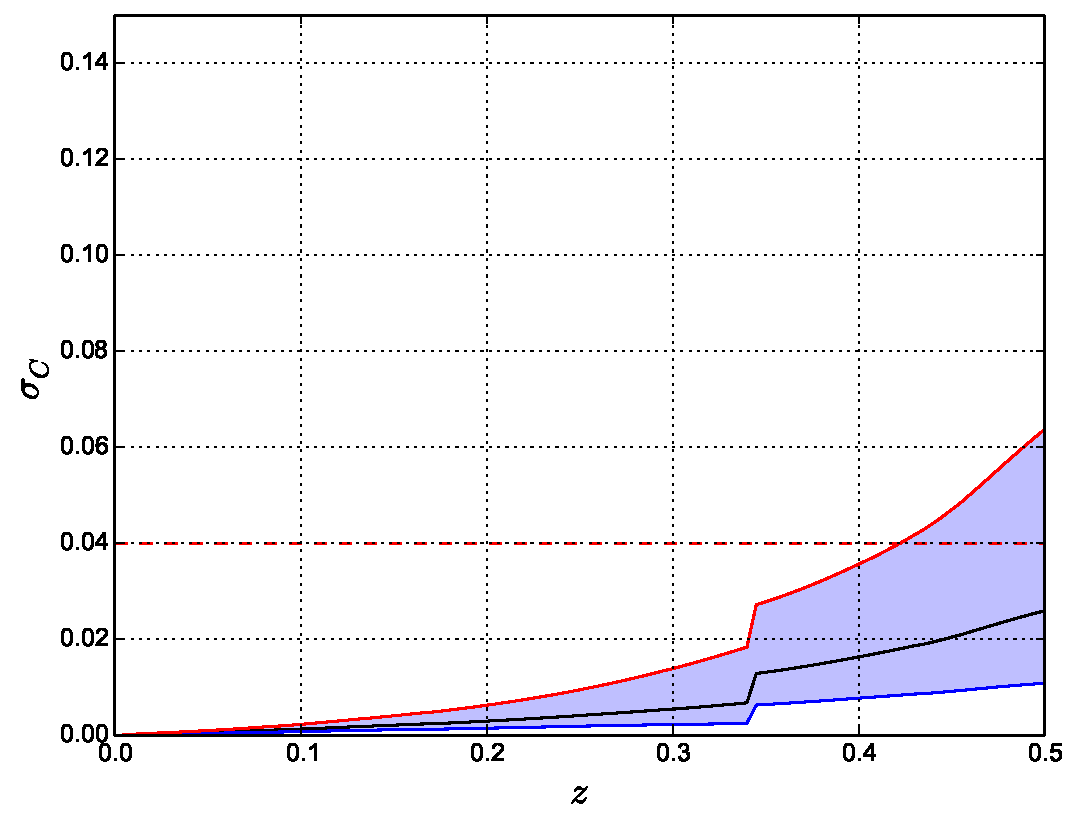
\includegraphics[width=0.49\linewidth]{sigc_lsstpg_wide_60.pdf}}
\subfigure[\code{SMTN-002} -- standard visits]{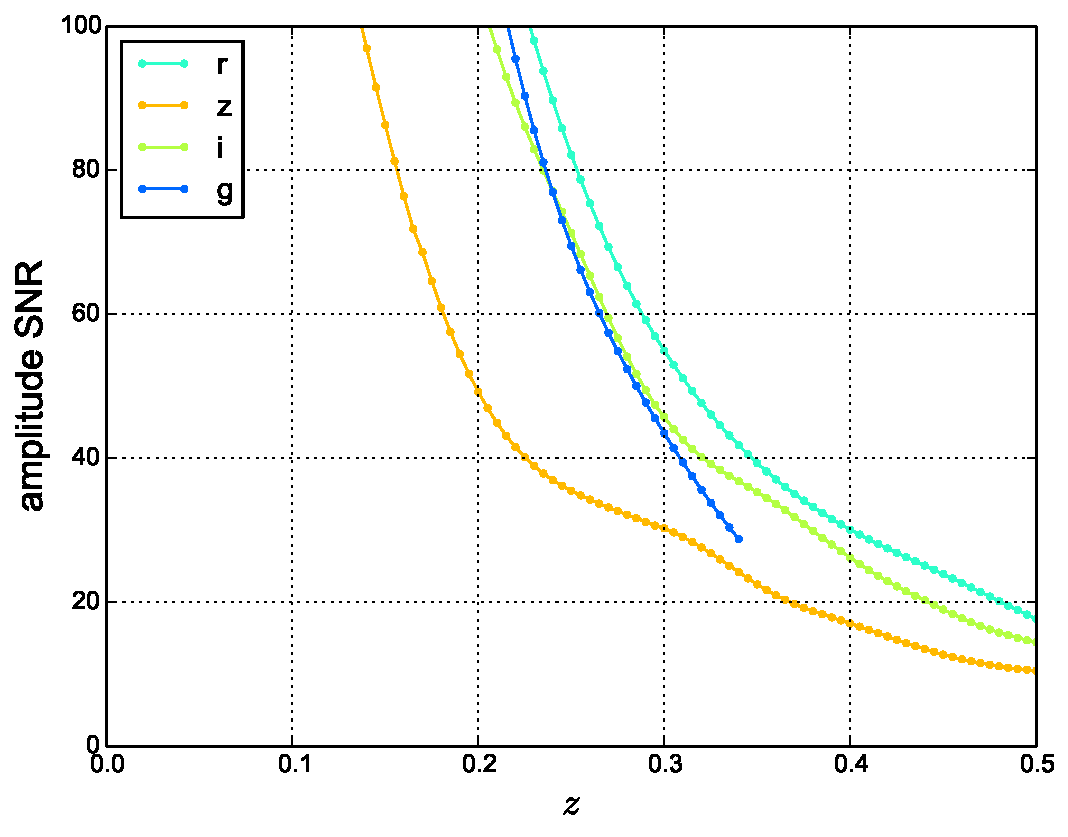
\includegraphics[width=0.49\linewidth]{snr_lsstpg_wide_30.pdf}}
\subfigure[\code{SMTN-002} -- deeper]{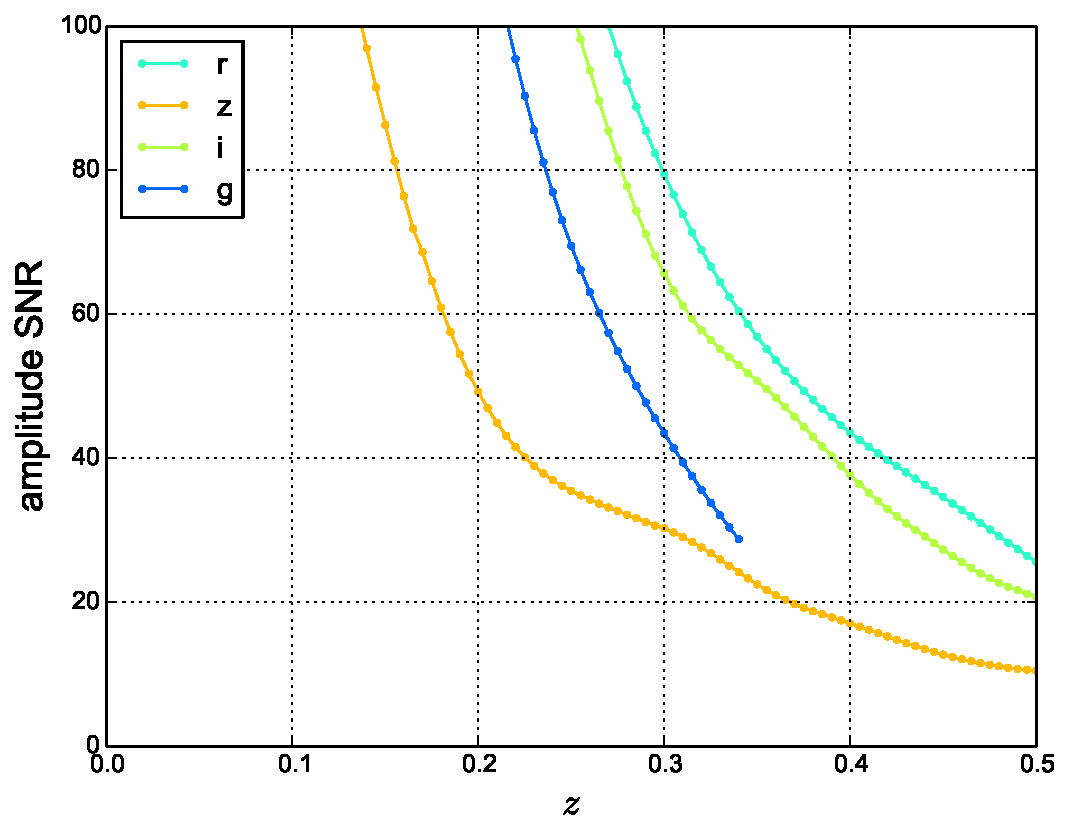
\includegraphics[width=0.49\linewidth]{snr_lsstpg_wide_60.pdf}}
\end{center}
\caption{Upper panels: $\sigma_C$ (shot noise only) obtained on the
  standard fields as a function of redshift.  On the left, for the
  standard 30-s visits and a 4 day cadence. On the right, we double
  the exposure times in $r$ and $i$.  (same cadence).  Lower panels:
  SNR obtained on the light curve amplitude, as a function of
  redshift.}
\label{fig:sigc_vs_z_4_day_cadence_wide}
\end{figure*}


\begin{table*}
\begin{center}
\caption{A nominal scenario for the wide that allows to build a SN
  sample complete up to $z \sim 0.4$.}
\label{tab:nominal_scenario_DDF}
\begin{tabular}{l|cccc}
\hline
\hline
              & $g$ & $r$ & $i$ & $z$ \\
\hline 
$T_{exp}$      & 30       &   30    &  30        & 30       \\
$m_{5\sigma}$  &  24.83   &  24.35   &  23.88    &  23.30   \\
cadence       &  \multicolumn{4}{c}{3 days} \\
Target amplitude SNR & $>30$ & $>40$ & $>30$ & $>20$ \\
\hline
\end{tabular}
\end{center}
\end{table*}




We have produced the same plots the main (shallow, wide)
survey. Figure \ref{fig:m5_cadence_limits_wide} shows the cadence {\em
  vs.}  $m_{5\sigma}$ plane for the wide survey.  The red stars
indicates the depth to attain, with a 4-day observer-frame cadence
(22.9, 22.5, 22.3 in $r, i, $ and $z$ respectively).

The red crosses indicate what we get from \code{Minion\_1016} for 3
wide fields. If we target a survey complete up to $z_{lim} \sim 0.4$
we find that:
\begin{itemize}
  \item in $r, i, $ and $z$ the cadence is too high ($\sim 10$ w.r.t 4 days observer frame)
  \item in all bands, the cadence is extremely variable from field to
    field (and from one year to another).
  \item in $r$ and $i$, we go deep enough with the standard visits;
  \item in $z$, we are not deep enough. It is likely that most $z$
    band observations are taken with the moon up. For a SN survey targeting 
    $z_{lim} = 0.4$, we need to either increase the exposure time in $z$, and 
    observe also when the moon is down.    
  \item in $g$, the cadence is extremely variable. This is ok for SNe
    close to $z_{lim}$.  However, this reduces our ability to catch
    nearby SNe.
\end{itemize}

\begin{figure*}[t]
\begin{center}
\subfigure[$g$]{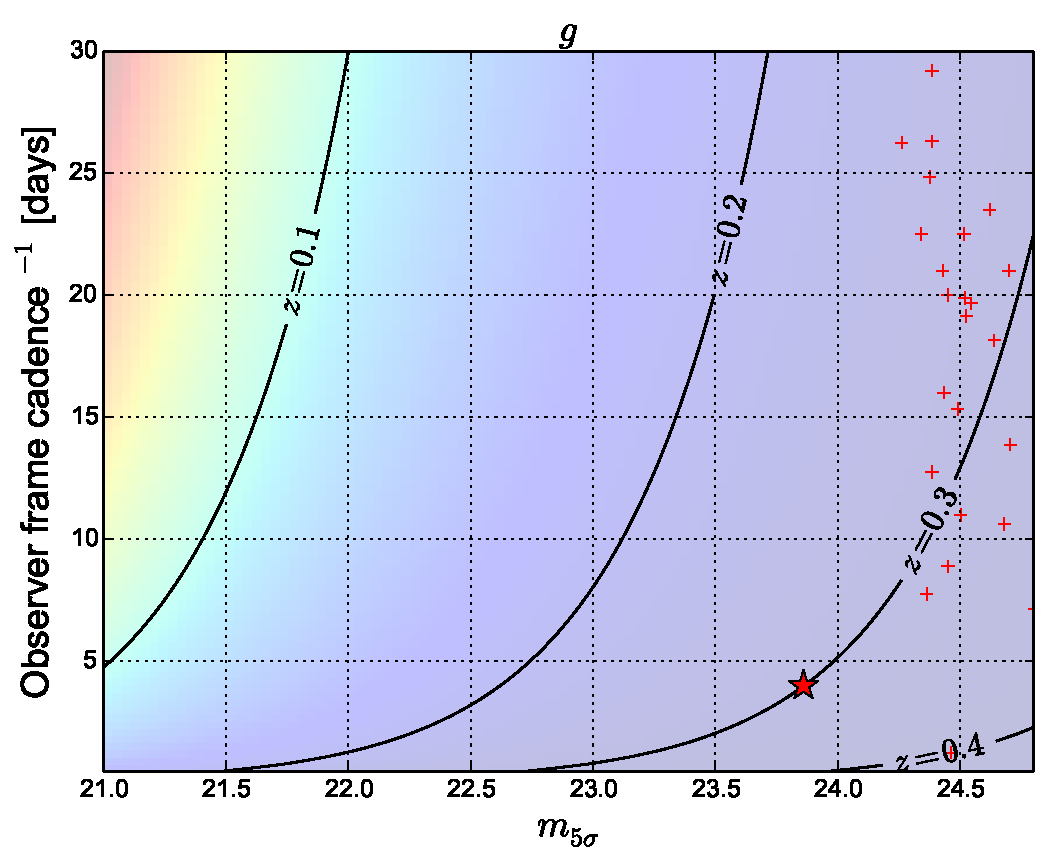
\includegraphics[width=0.48\linewidth]{m5_cadence_limits_wide_g.pdf}}
\subfigure[$r$]{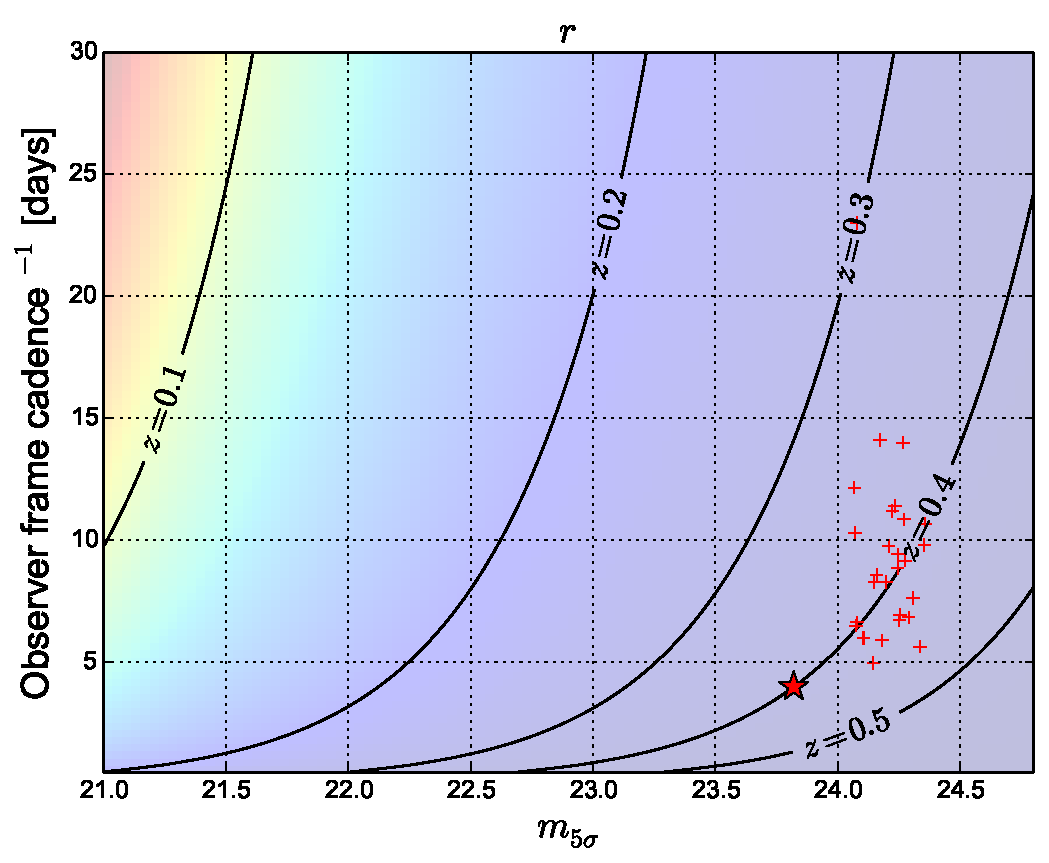
\includegraphics[width=0.48\linewidth]{m5_cadence_limits_wide_r.pdf}}\\
\subfigure[$i$]{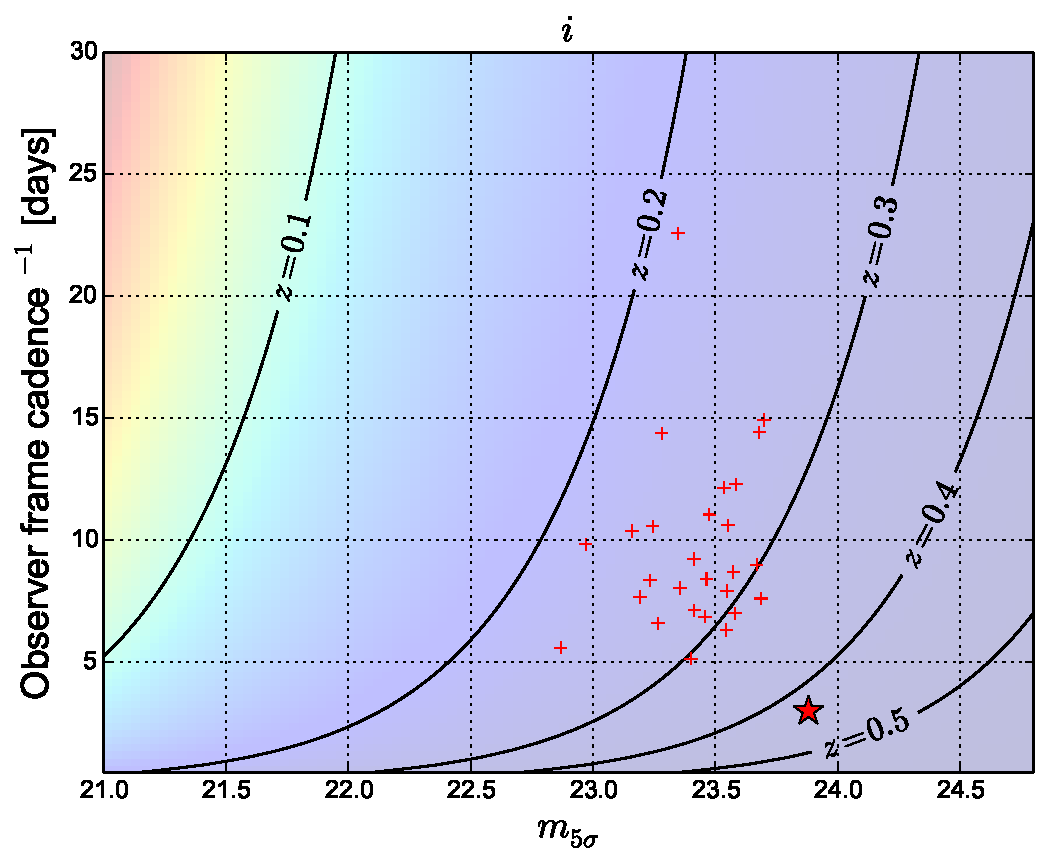
\includegraphics[width=0.48\linewidth]{m5_cadence_limits_wide_i.pdf}}
\subfigure[$z$]{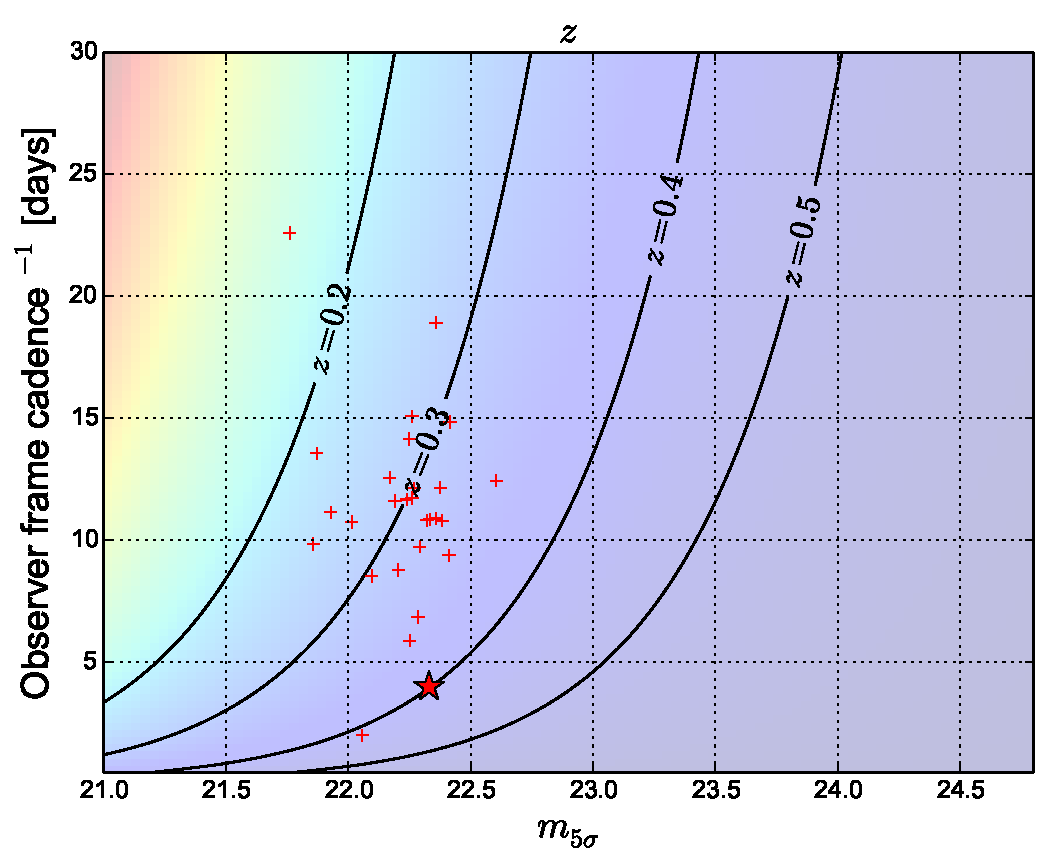
\includegraphics[width=0.48\linewidth]{m5_cadence_limits_wide_z.pdf}}
\caption{The cadence {\em vs.} depth requirements for the Wide survey,
  in the $g, r, i$ and $z$-bands. The color scale corresponds to the
  metric described in equation \ref{eqn:global_metric}.  The lines are
  the contour-levels computed for the limits indicated on table
  \ref{tab:cadence_depth_limit}. To fulfill the SNR requirements at a
  given redshift, one has to be {\em below} the corresponding
  line. The stars indicate an ambitious -- but attainable -- goal for
  a DDF survey.  The red crosses show what the survey can currently
  deliver according to \code{Minion\_1016}.}
\label{fig:m5_cadence_limits_wide}
\end{center}
\end{figure*}

\begin{figure*}[t]
  \begin{center}
    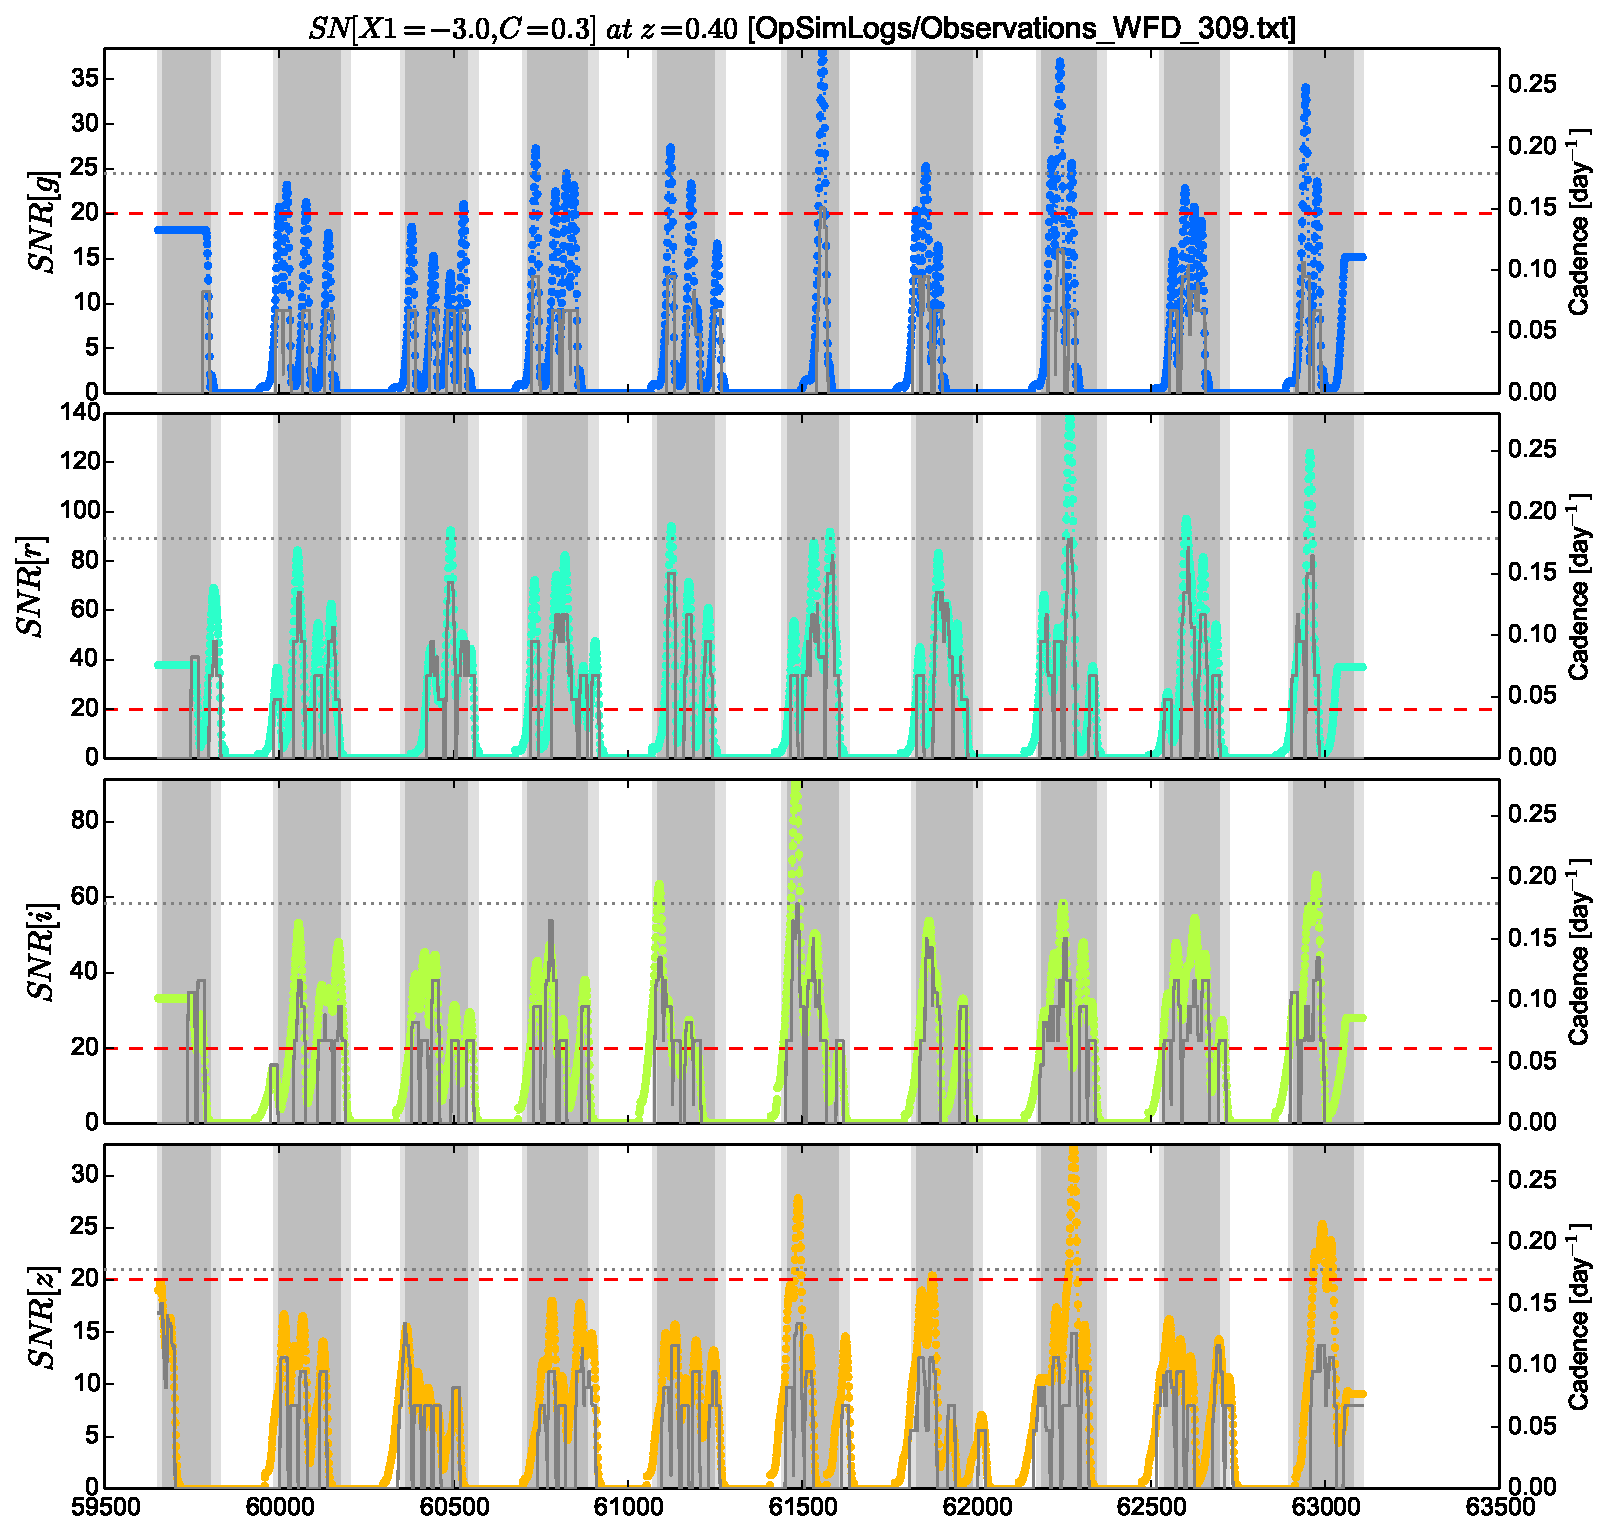
\includegraphics[width=\linewidth]{metric_WFD_309.pdf}
    \caption{Colored lines: the SNR of the estimated amplitude of a
      $[X_1=-2, C=0.25]$ SN~Ia at a redshift $z = 0.4$ as a function of
      peak MJD, computed for the \code{Minion\_1016} cadence and depth
      for field \#309. The SNR target is shown with the dashed red
      line.  Thin gray lines: the cadence delivered in that band,
      averaged in 30-day a sliding window.  The cadence target is
      represented as a dotted line. The plot extends over the 10 years
      of survey operations. The gray area corresponds to the search
      seasons for that field. The light gray area corresponds to the
      margins for which the SN has no points before (resp after)
      peak.}
    \label{fig:snr_metric_wide}
  \end{center}
\end{figure*}

On figure \ref{fig:snr_metric_wide}, we show again the SNR of our
faint SN at $z_{lim} \sim 0.4$ as a function of SN peak MJD in bands
$g, r, i$ and $z$. We see again that the depth in $z$ (and $g$) does
not yet allow to stay above a SNR of 20 over the duration of each
observing season.



% ----------------------------------------------------------------------

\section{Rolling Cadence on the wide survey}
\label{sec:rolling_cadence}

{\em [PG] to be written}

The basic idea of the rolling cadence is to gather the ten-year
observations of a WFD field into a smaller subset of seasons
(typically three). Since it was not possible to simulate such a
strategy with the OpSim version (v3.3.5) used to produce the \code{Minion\_1016}
file, we have fake a rolling cadence by merging subsets of three WFD
fields in a coherent way. The basic principle is the following. Let us
consider three sets of observations corresponding to WFD fields,
namely \fia, \fib, and \fic, and a merging factor m
(0$\leq$m$\leq$1).  Observations corresponding to the rolling cadence
will be denoted \fiap, \fibp, and \ficp. The first season is kept
untouched. Observations related to the second season (and also to
seasons 5 and 8) of \fiap~are composed
of those of \fia~plus m fraction of observations of \fib~plus m fraction
of observations of \fic. Observations of \fibp~and \ficp~are comprised of
the remaining observations of \fib~and \fic. The same procedure is
adopted for the following seasons, with the following permutation :
\fia (\fiap) $\rightarrow$ \fib (\fibp) (season 3, 6 and 9) and \fib (\fibp)
$\rightarrow$ \fic (\ficp) (season 4, 7, and 10). A summary of the combinations
is given in  table \ref{tab:rolling_cadence}. We have made slices of
the (ra,dec) area corresponding to the WFD survey to choose the fields
to be merged. Each ra slice of two degrees was splitted in three dec
regions. The three closest fields (one from each part) were considered for the
merging. 

\begin{table}[t]
\begin{center}
\caption{Procedure used to merge WFD fields to fake a rolling
  cadence. The merging factor m was set to 0.8.}
\label{tab:rolling_cadence}
\begin{tabular}{c|l}
\hline
\hline
    season   &      Observations \\
\hline
       & \fiap = \fia \\
    1 & \fibp = \fib \\
       & \fic = \fic \\
\hline
               & \fiap = \fia+m*\fib+m*\fic \\
    2, 5, 8 & \fibp = (1-m)*\fib \\
               & \ficp = (1-m)*\fic \\
\hline
               & \fiap = (1-m)*\fia \\
    3, 6, 9 & \fibp = \fib +m*\fia+m*\fic\\
              & \ficp = (1-m)*\fic \\
\hline
                 & \fiap = (1-m)*\fia\\
    4, 7, 10 & \fibp = (1-m)*\fib \\
                 & \ficp = \fic +m*\fia+m*\fib\\
\hline
\end{tabular}
\end{center}
\end{table}

The resulting observing strategy is given on figure
\ref{fig:rolling_strategy}. We have tried to merge fields in a coherent way. In addition to
elementary ajustments (such as the (ra,dec) values), we have performed
a reshuffling of observations corresponding to \fiap (seasons 2, 5,
and 8),\fibp (seasons 3, 6, and 9), and \ficp (seasons 4, 7, and
10). For each season and each band, we aimed at distributing
observations while keeping good observing conditions that is an
airmass value between 1 and 1.5 (this upper limit was imposed by OpSim
when producing the \code{Minion\_1016} cadence), a Moon phase lower
than 60\% and a Moon zenith distance higher than 85$^°$. These last
two conditions ensure that the brightness of the
sky is acceptable. Observations at twilight were not retained.

\begin{figure*}[t]
  \begin{center}
    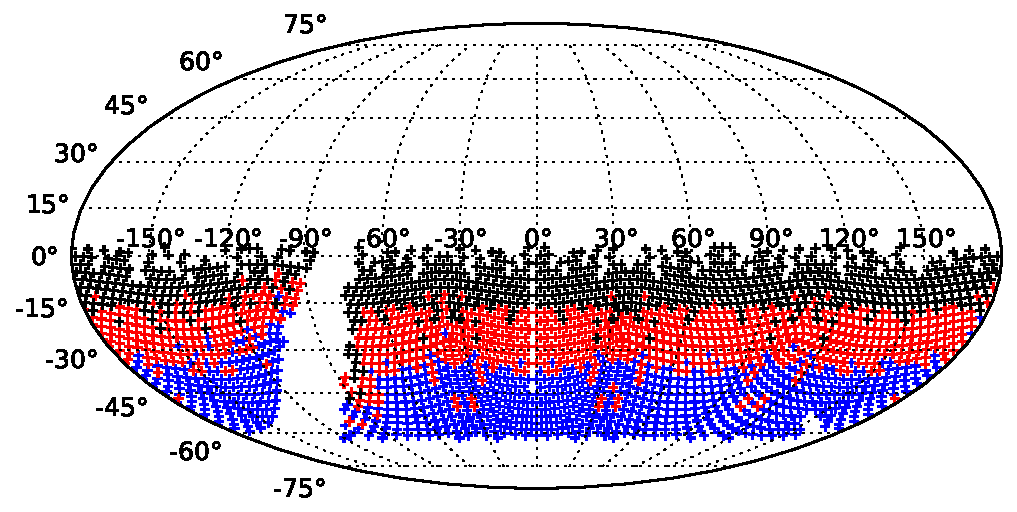
\includegraphics[width=\linewidth]{figures/Rolling_fields.pdf}
    \caption{Observing strategy corresponding to the rolling
      cadence. Blue, red and black crosses correspond to fields
      observed during seasons (2,5,8), (3,6,9), and
      (4,7,10), respectively.}
    \label{fig:rolling_strategy}
  \end{center}
\end{figure*}



% ----------------------------------------------------------------------

\section{Conclusions}
\label{sec:conclusions}

We have presented lightweight metrics to assess whether a given
cadence permits to build a redshift-limited sample up to a given
redshift $z_{lim}$, without having to resort to an extensive
simulation.

We have presented design guidelines for the wide and deep LSST SN
surveys and discussed requirements on the survey depth and cadence.

We have evaluated the \code{Minion\_1016} cadence, on a series of DDF
and wide fields. On the DDF fields, we have found that the current
cadence yields a SN survey complete up to $z \sim 0.65$.  This is
comparable to what was obtained with SNLS in the 2000's but well below
what should be an ambitious goal for LSST (produce a redshift limited
SN~Ia Hubble diagram up to $z_{lim} \sim 1$).

\FIXME{Conclusion on the main survey depends on what we obtain from
  the wide rolling cadence.}

The results presented here should be taken with a bit of caution.  As
we discuss in appendix \ref{sec:lsst_instrument_models}, and shown on
figure \ref{fig:lsst_model_summary}, the assessment of the instrument
throughput and of the average observing conditions have been recently
revised, and this revision has a very significant impact on the
expected survey depth (almost half a magnitude per standard visit).

Furthermore, the average observing conditions used in
\code{Minion\_{1016}} seem to be quite pessimistic.  In particular,
the \code{Minion\_{1016}} sky brightness is probably too bright,
especially in the $y$-band.


% \begin{itemize}
% \item on the DDF fields, the survey is complete up to $z \sim
%   0.65$. This is comparable to what was obtained with SNLS in the
%   2000's but well below what should be an ambitious goal for LSST
%   (produce a redshift limited SN~Ia Hubble diagram up to $z_{lim} \sim
%   1$).

% \item on the DDF fields, increasing the duration of the search seasons
%   from 4.5 months to 6 months would allow to gain tremendously in
%   statistics (almost a factor 2) at high redshift.
  
% \item on the Wide fields, the redshift limit is of about $z \sim
%   0.3$. A more ambitious target is rather $z_{lim} \sim 0.4$.  In the
%   $g$-band, the regularity of the cadence should be improved.

% \item we have shown that, by tweaking the cadence, one can reach a
%   $z_{lim}$ of 0.9 for the DDF fields and $z_{lim} \sim 0.4$ on the
%   Wide, in the same observing time budget.

% \item it remains to be proven that these cadences can be reached
%   within the constraints of the survey operations, as they are
%   implemented in {\tt OpSim}.  We suggest implementing, in the OpSim
%   scheduler, a dynamic scheduling algorithm based on the metrics
%   discussed above.  
  
%   To give orders of magnitudes, a reasonable target is a cadence of 4
%   restframe days at the median redshift of the wide and deep surveys.
%   This corresponds to an observer frame cadence of $\sim 5.2$ (resp
%   6.8) days on the wide and the DDF respectively.

% \item finally, the results presented here should be taken with a bit
%   of caution.  As we discuss in appendix
%   \ref{sec:lsst_instrument_models}, and shown on figure
%   \ref{fig:lsst_model_summary}, the assessment of the instrument
%   throughput and of the average observing conditions have been
%   recently revised, and this revision has a very significant impact on
%   the expected survey depth (almost half a magnitude per standard
%   visit).  

%   Furthermore, the average observing conditions used in
%   \code{Minion\_{1016}} seem to be quite pessimistic.  In particular,
%   the \code{Minion\_{1016}} sky brightness is probably too bright,
%   especially in the $y$-band.
% \end{itemize}

The results presented in this note will be updated as revised OpSim
cadences become available.


% ----------------------------------------------------------------------

\subsection*{Acknowledgments}

% Here is where you should add your specific acknowledgments, remembering that some standard thanks will be added via the \code{acknowledgments.tex} and \code{contributions.tex} files.

% % 
This is the text imported from \code{acknowledgments.tex}, and will be replaced by some standard LSST DESC boilerplate at some point.
% 


% \input{contributions}

% {\it Facilities:} \facility{LSST}

% Include both collaboration papers and external citations:
\bibliography{lsstdesc,main}





\appendix

\section{LSST instrument models}
\label{sec:lsst_instrument_models}

We  have used  two instrument  models.  One  is based  on the  numbers
reported  in \cite[][LSE-40  hereafter]{LSE-40}.  We  report the  main
ingredients of this model in table \ref{tab:lse40}.

The other model is described in \cite[][hereafter
SMTN-002)]{SMTN-002}, which constitutes a preliminary update of
LSE-40.  The current version OpSim relies on SMTN-002. An we therefore
adopt this model as our reference. Key quantities of SMTN-002 are
listed in table \ref{tab:smtn002}.

We note that both models differ very significantly. In particular (1)
the throughput of SMTN-002 is almost 50\% lower.


\begin{table}
\begin{center}
\caption{LSE-40 model}
\label{tab:lse40}
\begin{tabular}{l|cccccc}
\hline 
\hline 
\multicolumn{7}{c}{{\bf General}} \\
\hline
Pixel size & \multicolumn{6}{r}{0.2 arcsec} \\
RO noise   & \multicolumn{6}{r}{9 $e^-$}    \\
\hline
\multicolumn{7}{c}{{\bf Zero Points @ X=1 [AB, fluxes in e$^-$/s]}} \\
\hline
           &  $u$ & $g$ & $r$ & $i$ & $z$ & $y$ \\
LSE-40     & 27.09 & 28.58 & 28.50 & 28.34 & 27.95 & 27.18 \\
snsim      & 27.05 & 28.59 & 28.53 & 28.38 & 27.99 & 27.22 \\
\hline
\multicolumn{7}{c}{{\bf median seeing [arcsec]}} \\
\hline
LSE-40 / snsim  &  0.77 &  0.73 &  0.70 &  0.67 &  0.65 &  0.63 \\
\hline
\multicolumn{7}{c}{{\bf Dark sky [AB mag / arcsec$^2$]}}   \\
\hline
LSE-40     & 22.92 & 22.27 & 21.20 & 20.47 & 19.59 & 18.63 \\
snsim      & 22.95 & 22.26 & 21.20 & 20.47 & 19.60 & 18.61 \\
\hline
\multicolumn{7}{c}{{\bf NEA [pixel$^2$]}}   \\
\hline
snsim (Moffat, $\beta=4.5$)     & 41.5  & 37.4  & 34.5  & 31.7 & 29.9  & 28.6  \\
\hline
\multicolumn{7}{c}{{\bf Limiting mag ($5 \sigma$), 30-s visit}}   \\
\hline
LSE-40                        & 24.22  &  25.15 &  24.74  &  24.38  &  23.80  &  22.93  \\
snsim (Moffat, $\beta=7$)     & 24.27  &  25.18 &  24.73  &  24.36  &  23.77  &  22.92  \\
\hline
\end{tabular}
\end{center}
\end{table}


\begin{table}
\begin{center}
\caption{SMTN-002 model}
\label{tab:smtn002}
\begin{tabular}{l|cccccc}
\hline 
\hline 
\multicolumn{7}{c}{{\bf General}} \\
\hline
Pixel size & \multicolumn{6}{r}{0.2 arcsec} \\
RO noise   & \multicolumn{6}{r}{9 $e^-$}    \\
\hline
\multicolumn{7}{c}{{\bf Zero Points @ X=1 [AB, fluxes in e$^-$/s]}} \\
\hline
           &  $u$ & $g$ & $r$ & $i$ & $z$ & $y$ \\
SMTN-002   & 26.50 & 28.30 & 28.13 & 27.79 & 27.40 & 26.58 \\
snsim      & 26.48 & 28.34 & 28.17 & 27.85 & 27.46 & 26.63 \\
\hline
\multicolumn{7}{c}{{\bf median seeing [arcsec]}} \\
\hline
SMTN-002 / snsim  &  0.92 &  0.87 &  0.83 &  0.80 &  0.78 &  0.76 \\
\hline
\multicolumn{7}{c}{{\bf Dark sky [AB mag / arcsec$^2$]}}   \\
\hline
SMTN-002   & 22.95 & 22.24 & 21.20 & 20.47 & 19.60 & 18.63 \\ %% line 1 of Table 2
snsim      & 22.98 & 22.23 & 21.19 & 20.46 & 19.60 & 18.61 \\
\hline
\multicolumn{7}{c}{{\bf NEA [pixel$^2$]}}   \\
\hline
snsim (Moffat, $\beta=7$)     & 58.8  & 52.7  & 48.0  & 44.7  & 42.6  & 40.5  \\
\hline
\multicolumn{7}{c}{{\bf Limiting mag ($5 \sigma$), 30-s visit}}   \\
\hline
SMTN-002                    &  23.60     &  24.83     &  24.38     &   23.92    &  23.35     &  22.44  \\
snsim (Moffat, $\beta=7$)   &  23.61     &  24.83     &  24.35     &   23.88    &  23.30     &  22.43  \\
\hline
\end{tabular}
\end{center}
\end{table}


\begin{figure}[t]
\begin{center}
\subfigure[LSE-40]{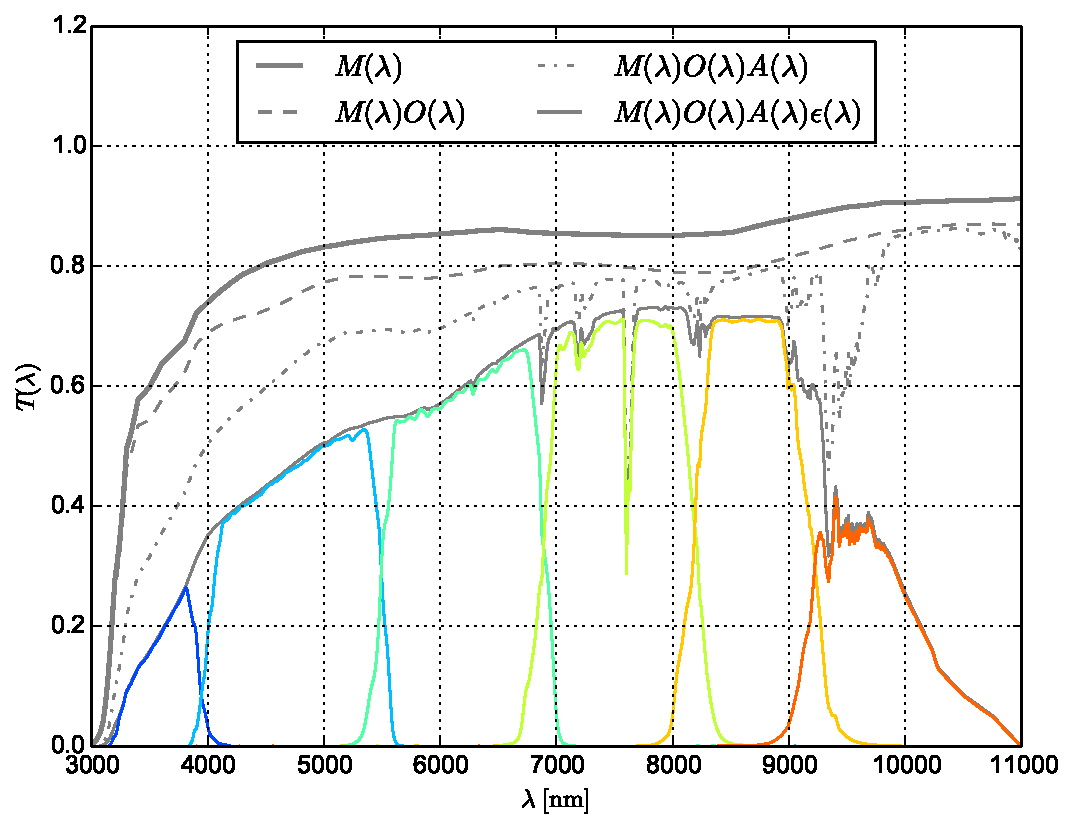
\includegraphics[width=0.45\linewidth]{lse_40_passbands.pdf}}
\subfigure[SMTN-002]{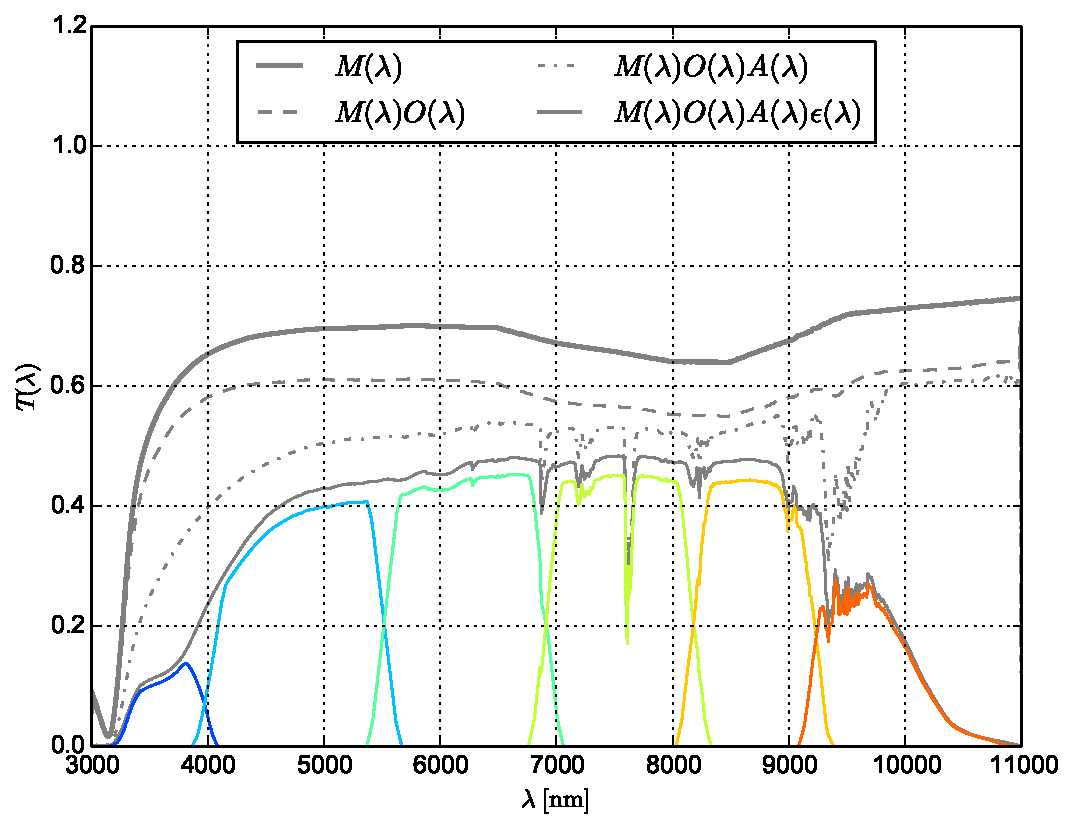
\includegraphics[width=0.45\linewidth]{smtn002_passbands.pdf}}
\caption{Instrument passbands}
\label{fig:throughput_comparison}
\end{center}
\end{figure}



\section{Additional figures}

\begin{figure}[t]
  \begin{center}
    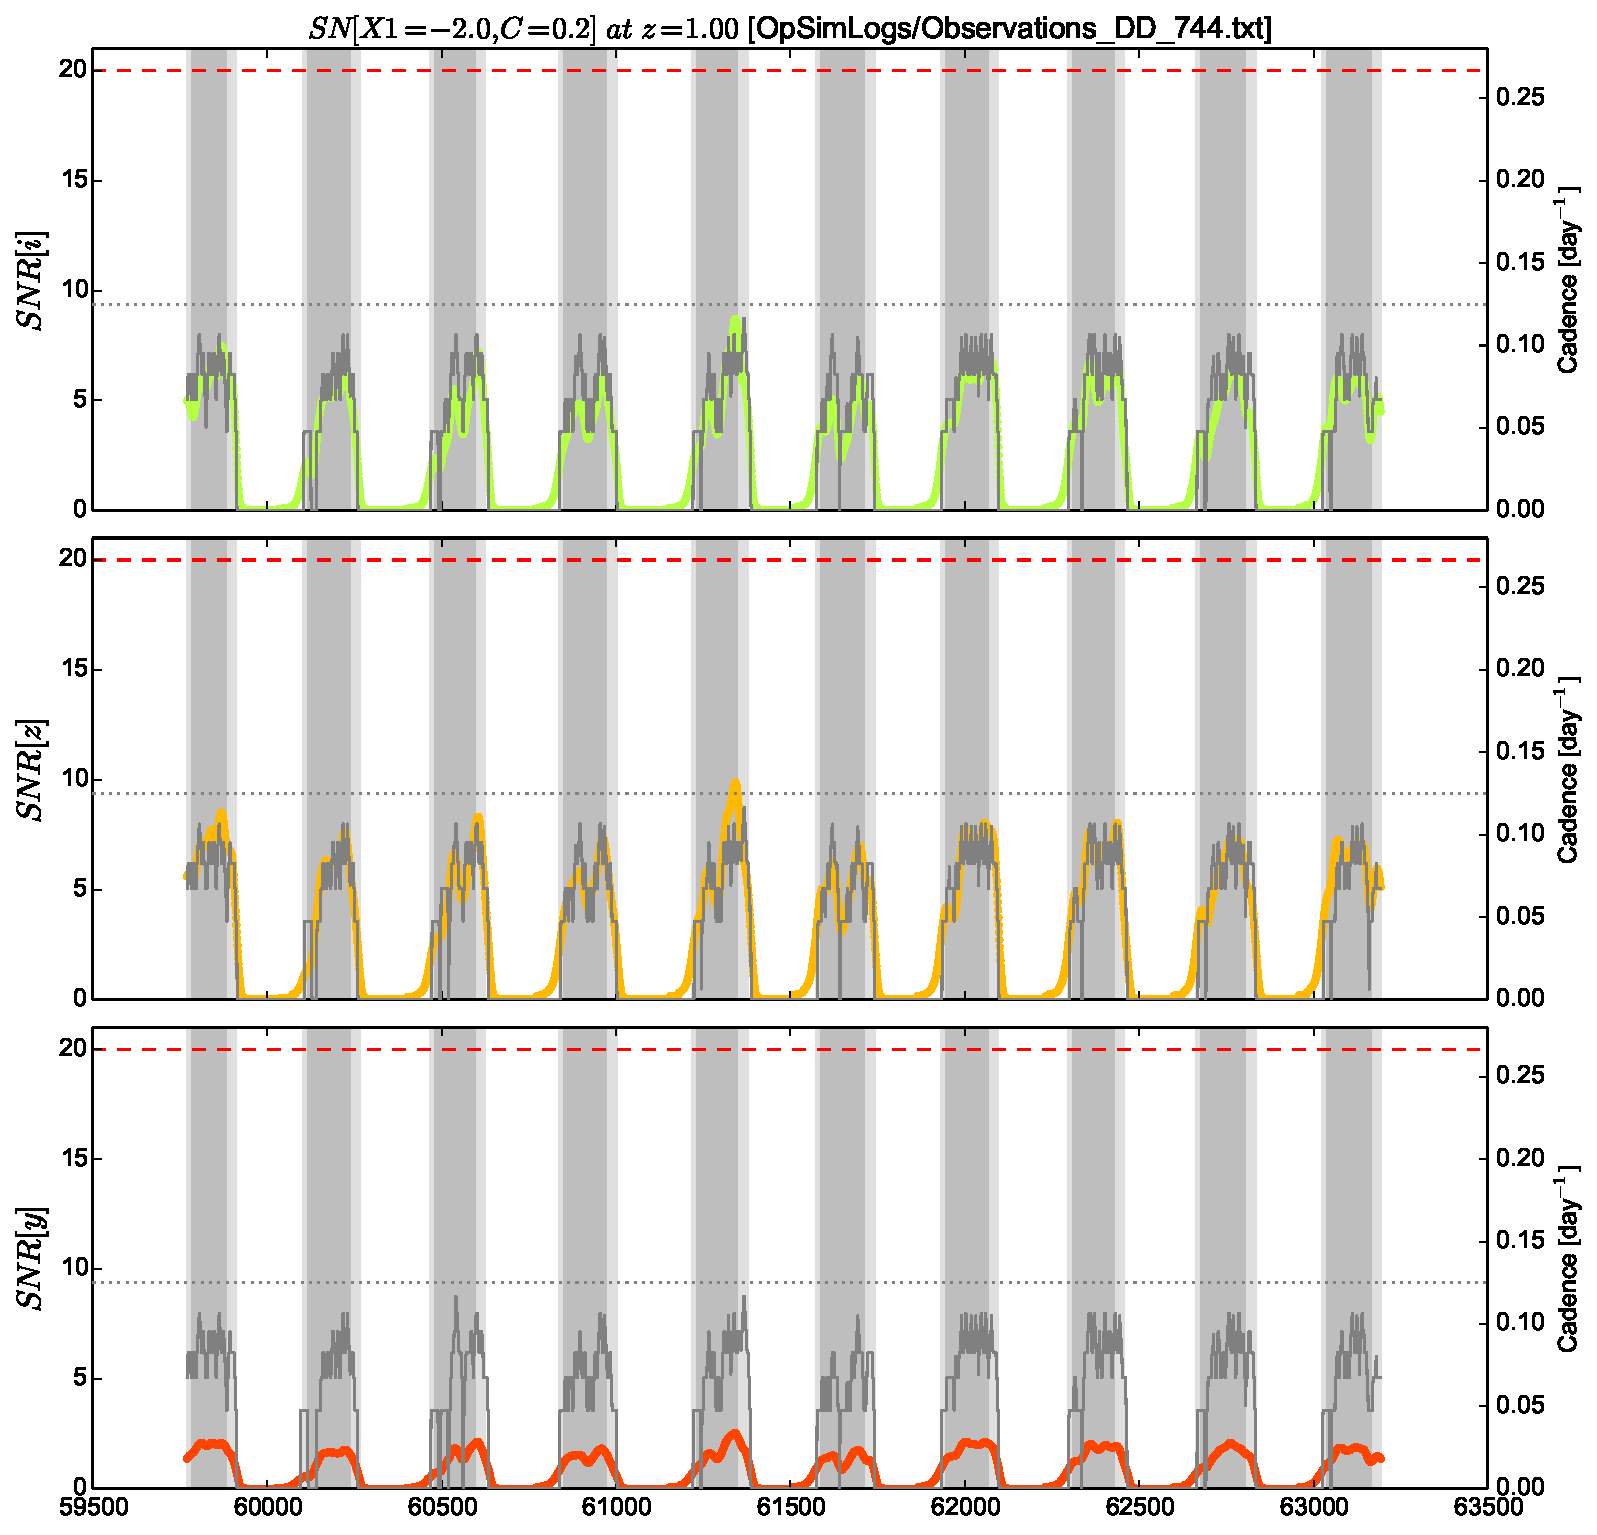
\includegraphics[width=\linewidth]{metric_DD_744.pdf}
    \caption{}
  \end{center}
\end{figure}


\begin{figure}[t]
  \begin{center}
    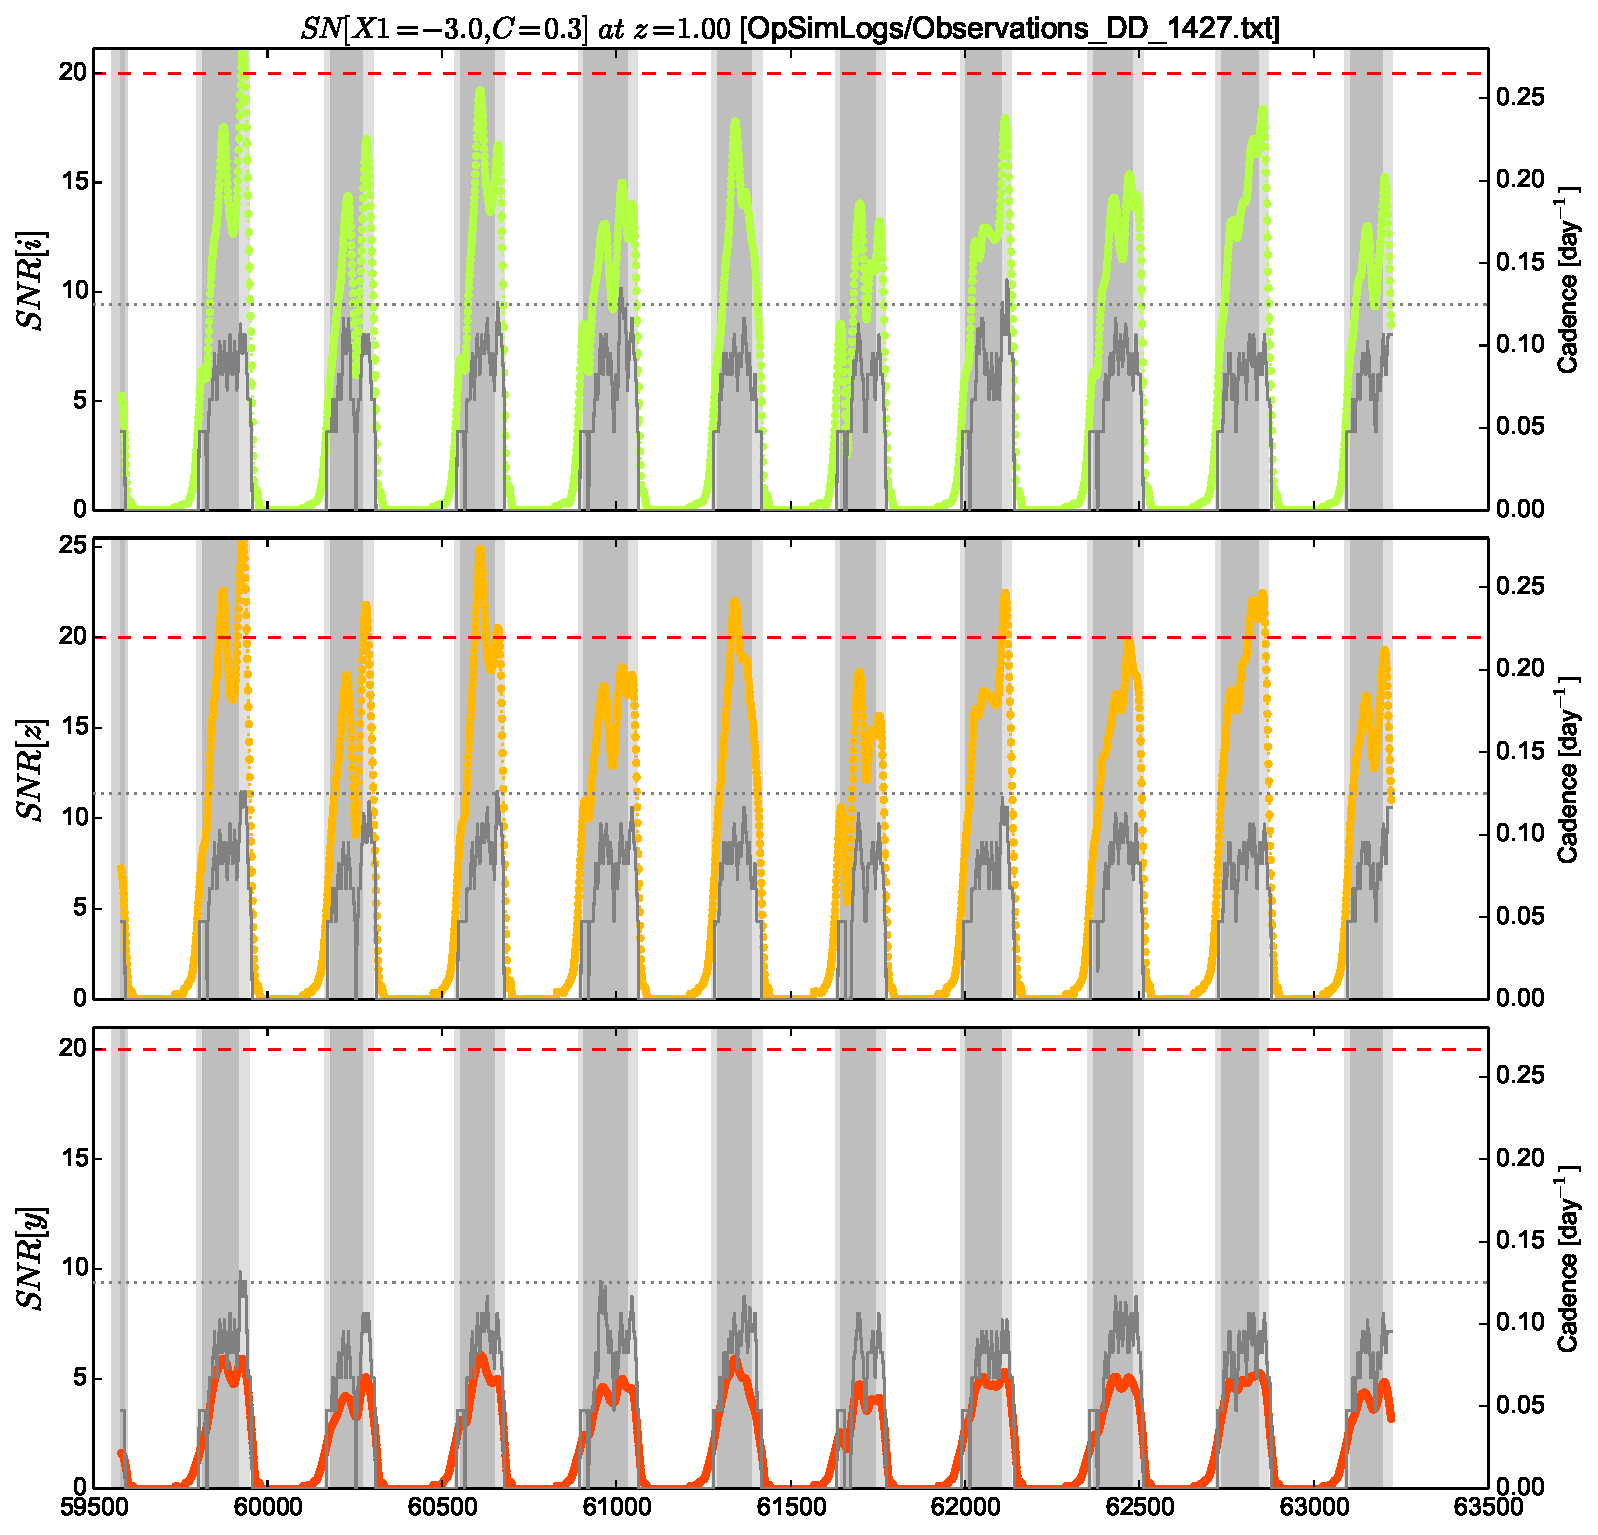
\includegraphics[width=\linewidth]{metric_DD_1427.pdf}
    \caption{}
  \end{center}
\end{figure}

\begin{figure}[t]
  \begin{center}
    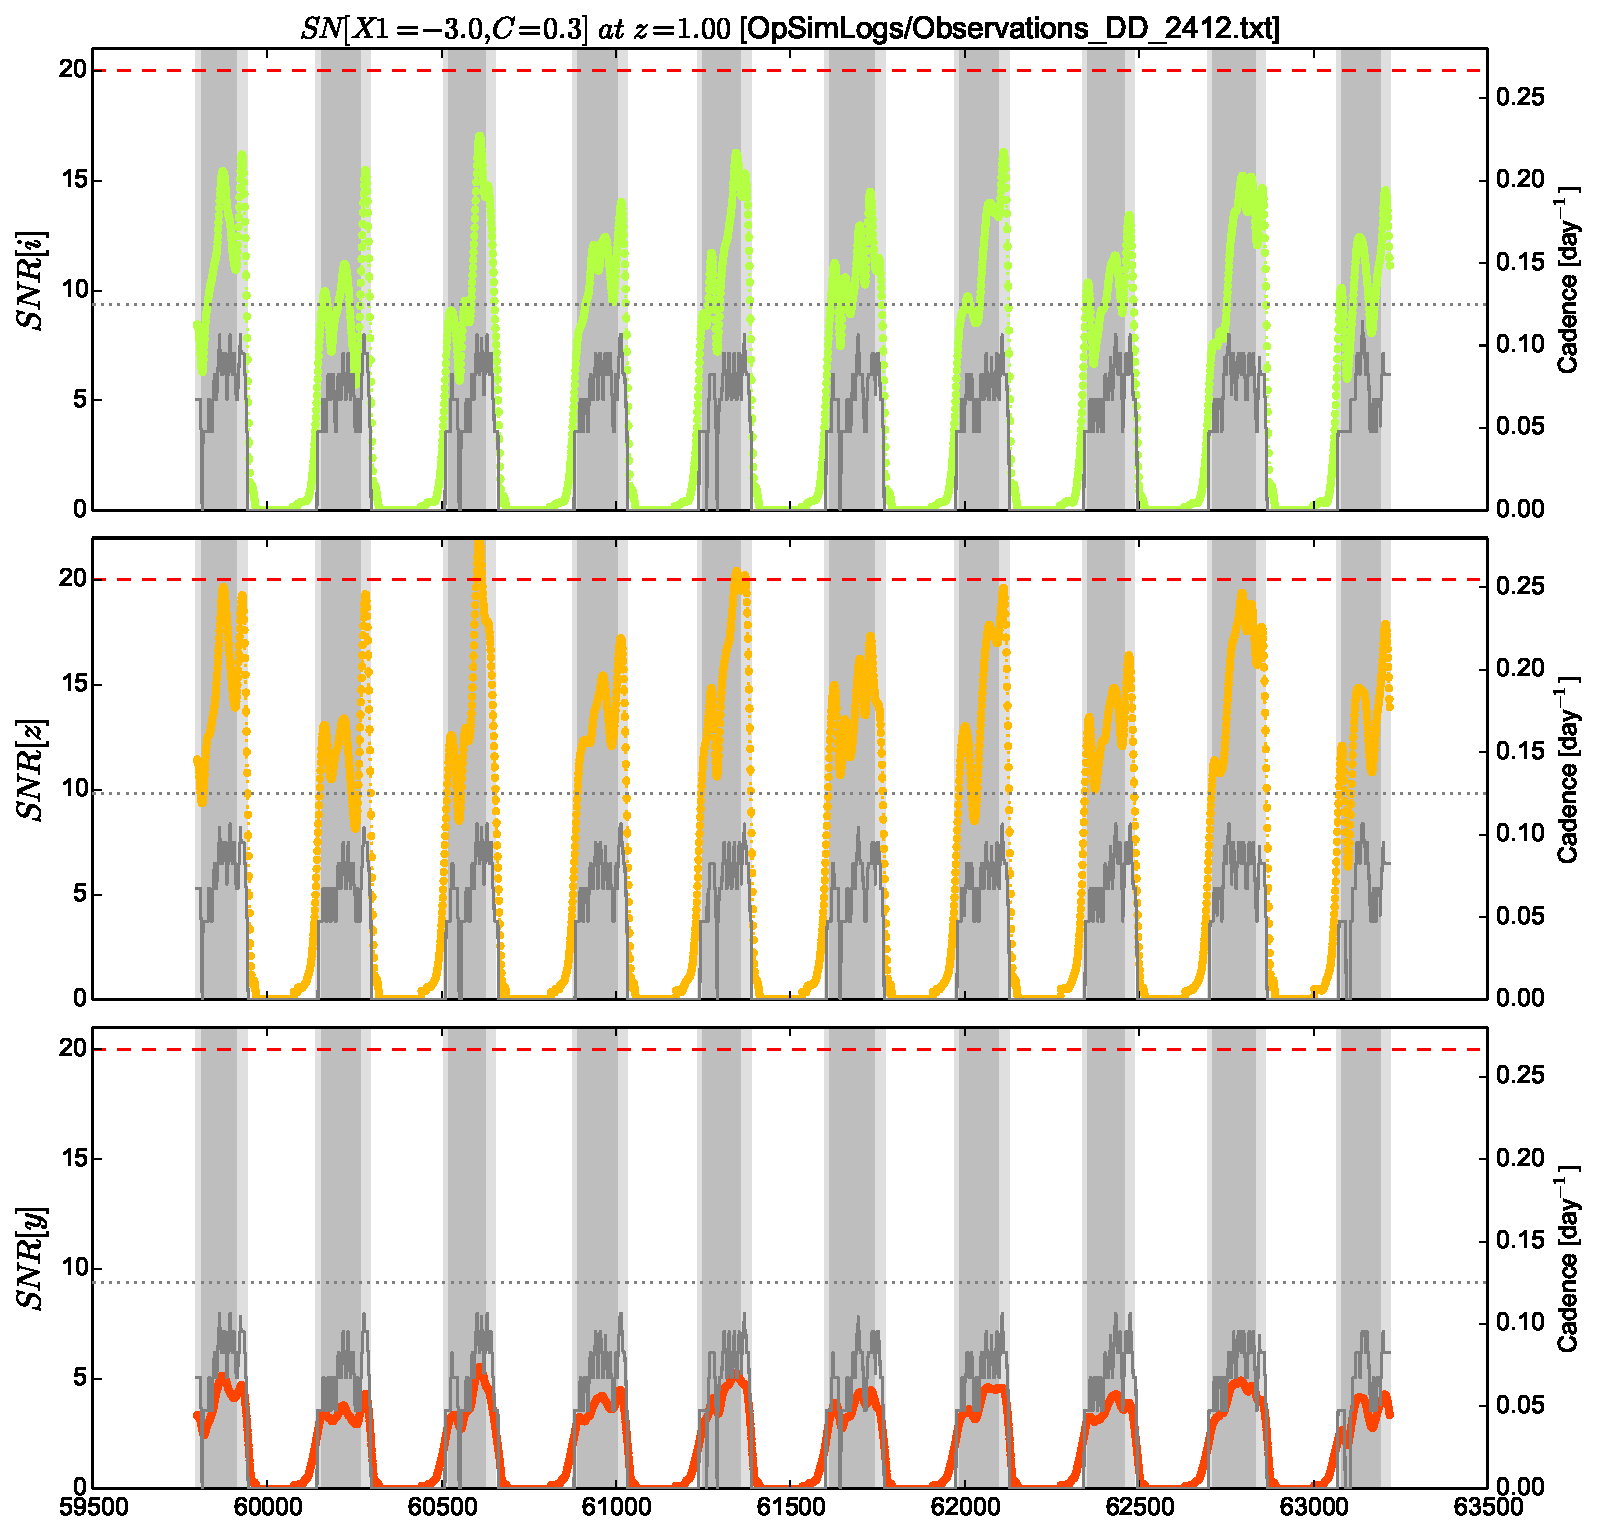
\includegraphics[width=\linewidth]{metric_DD_2412.pdf}
    \caption{}
  \end{center}
\end{figure}

\begin{figure}[t]
  \begin{center}
    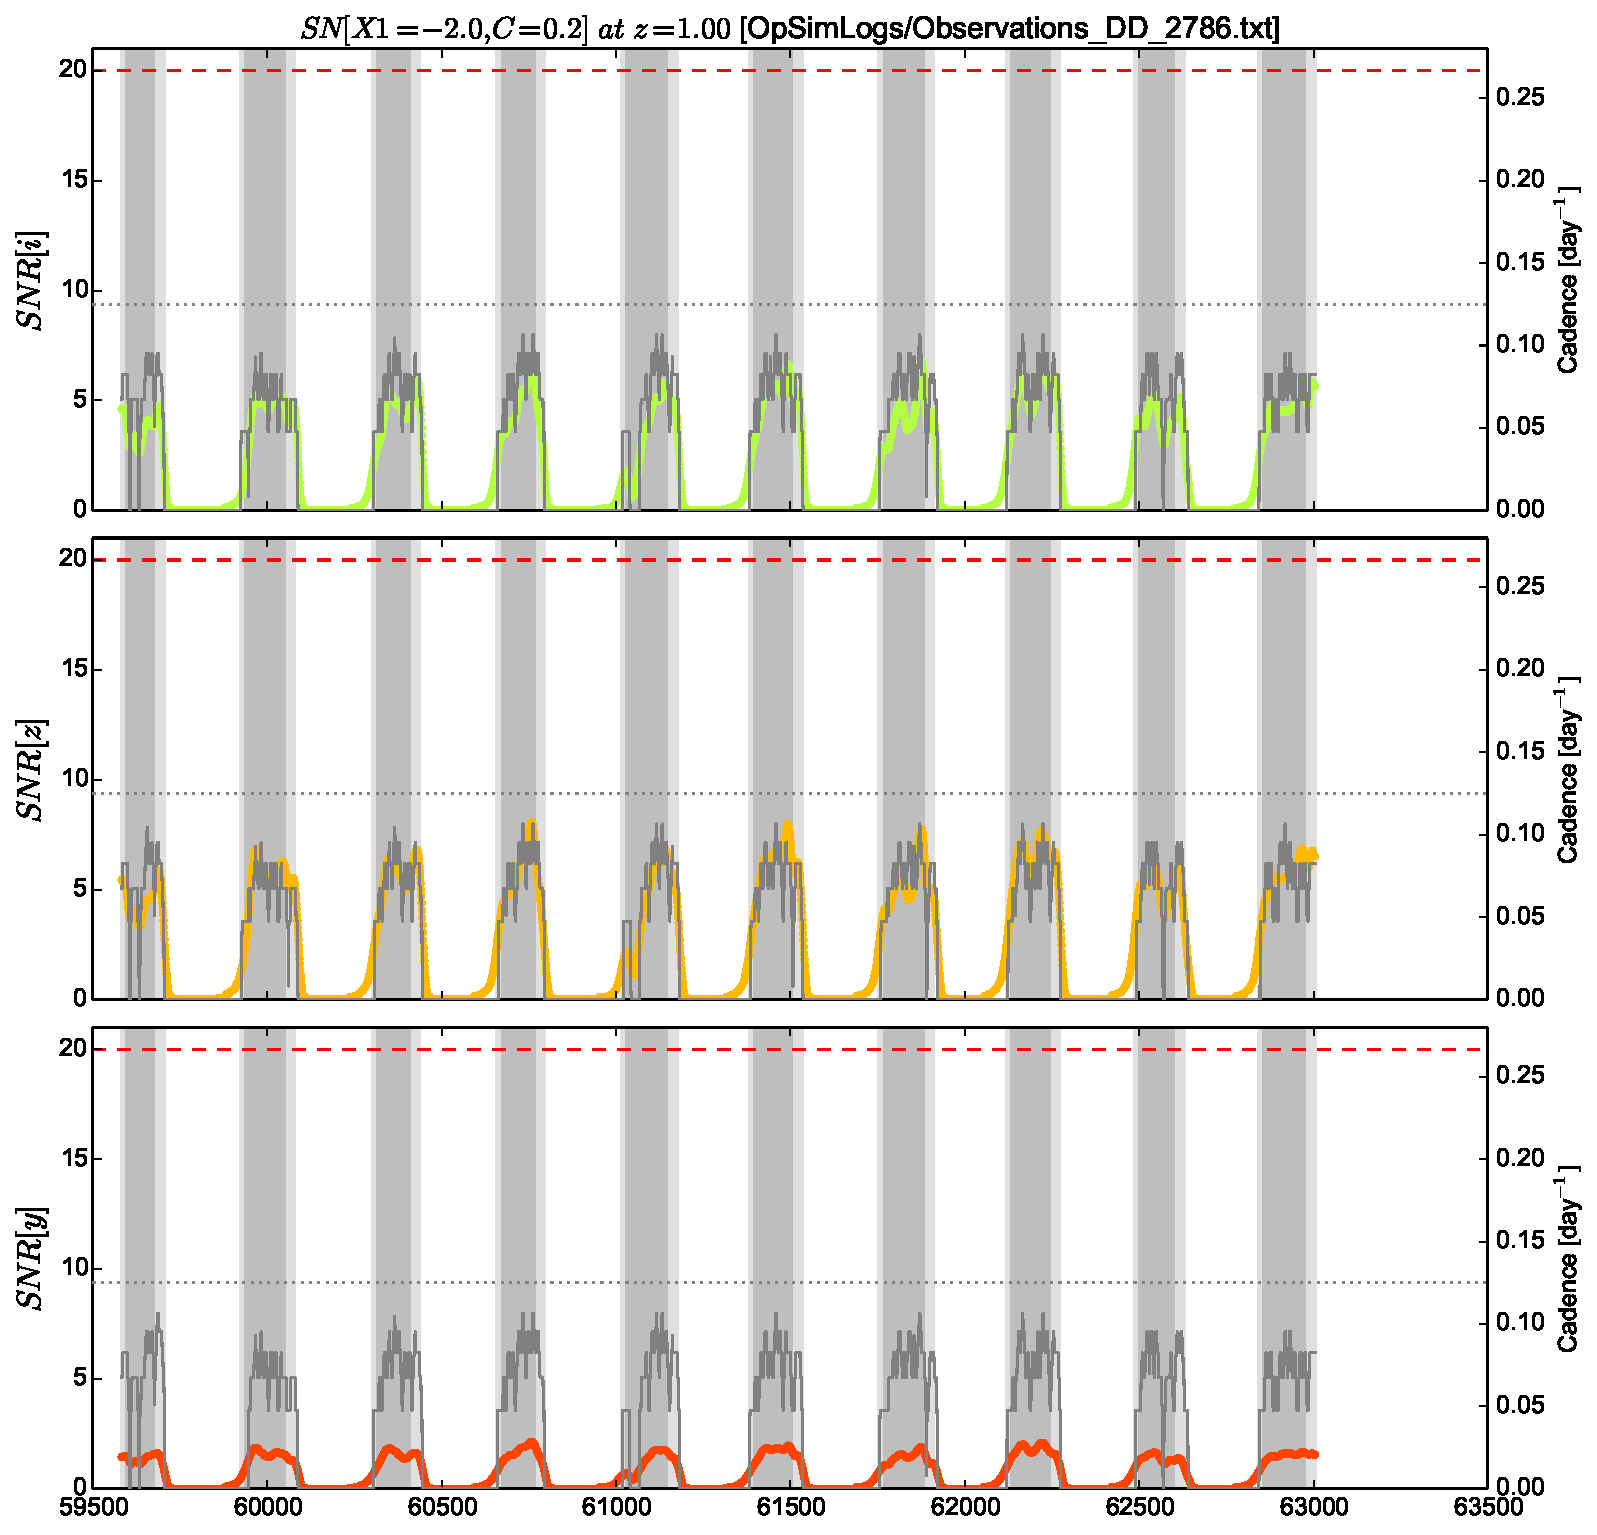
\includegraphics[width=\linewidth]{metric_DD_2786.pdf}
    \caption{}
  \end{center}
\end{figure}



\begin{figure*}[t]
  \begin{center}
    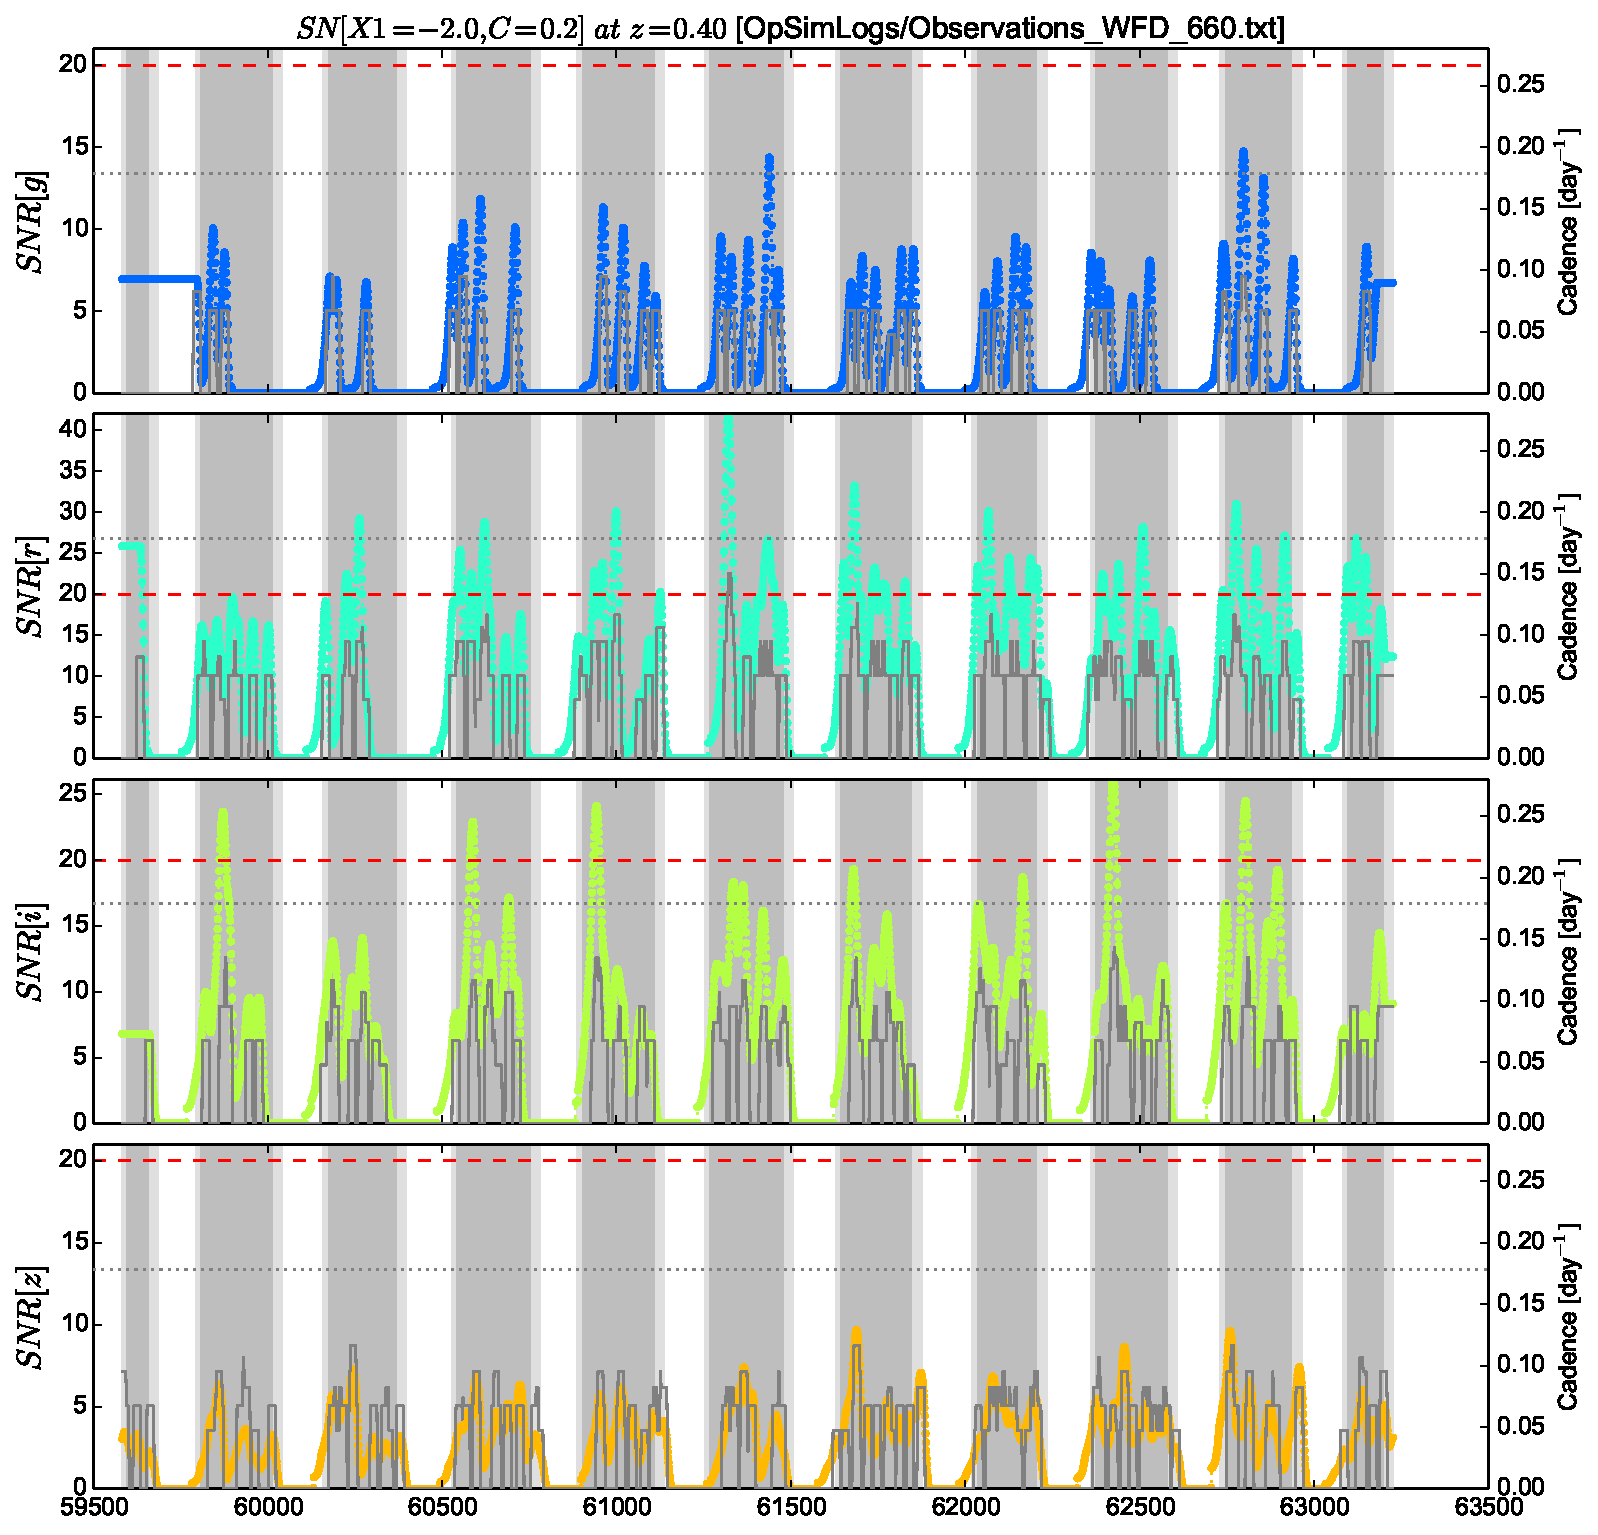
\includegraphics[width=\linewidth]{metric_WFD_660.pdf}
    \caption{}
  \end{center}
\end{figure*}

\begin{figure*}[t]
  \begin{center}
    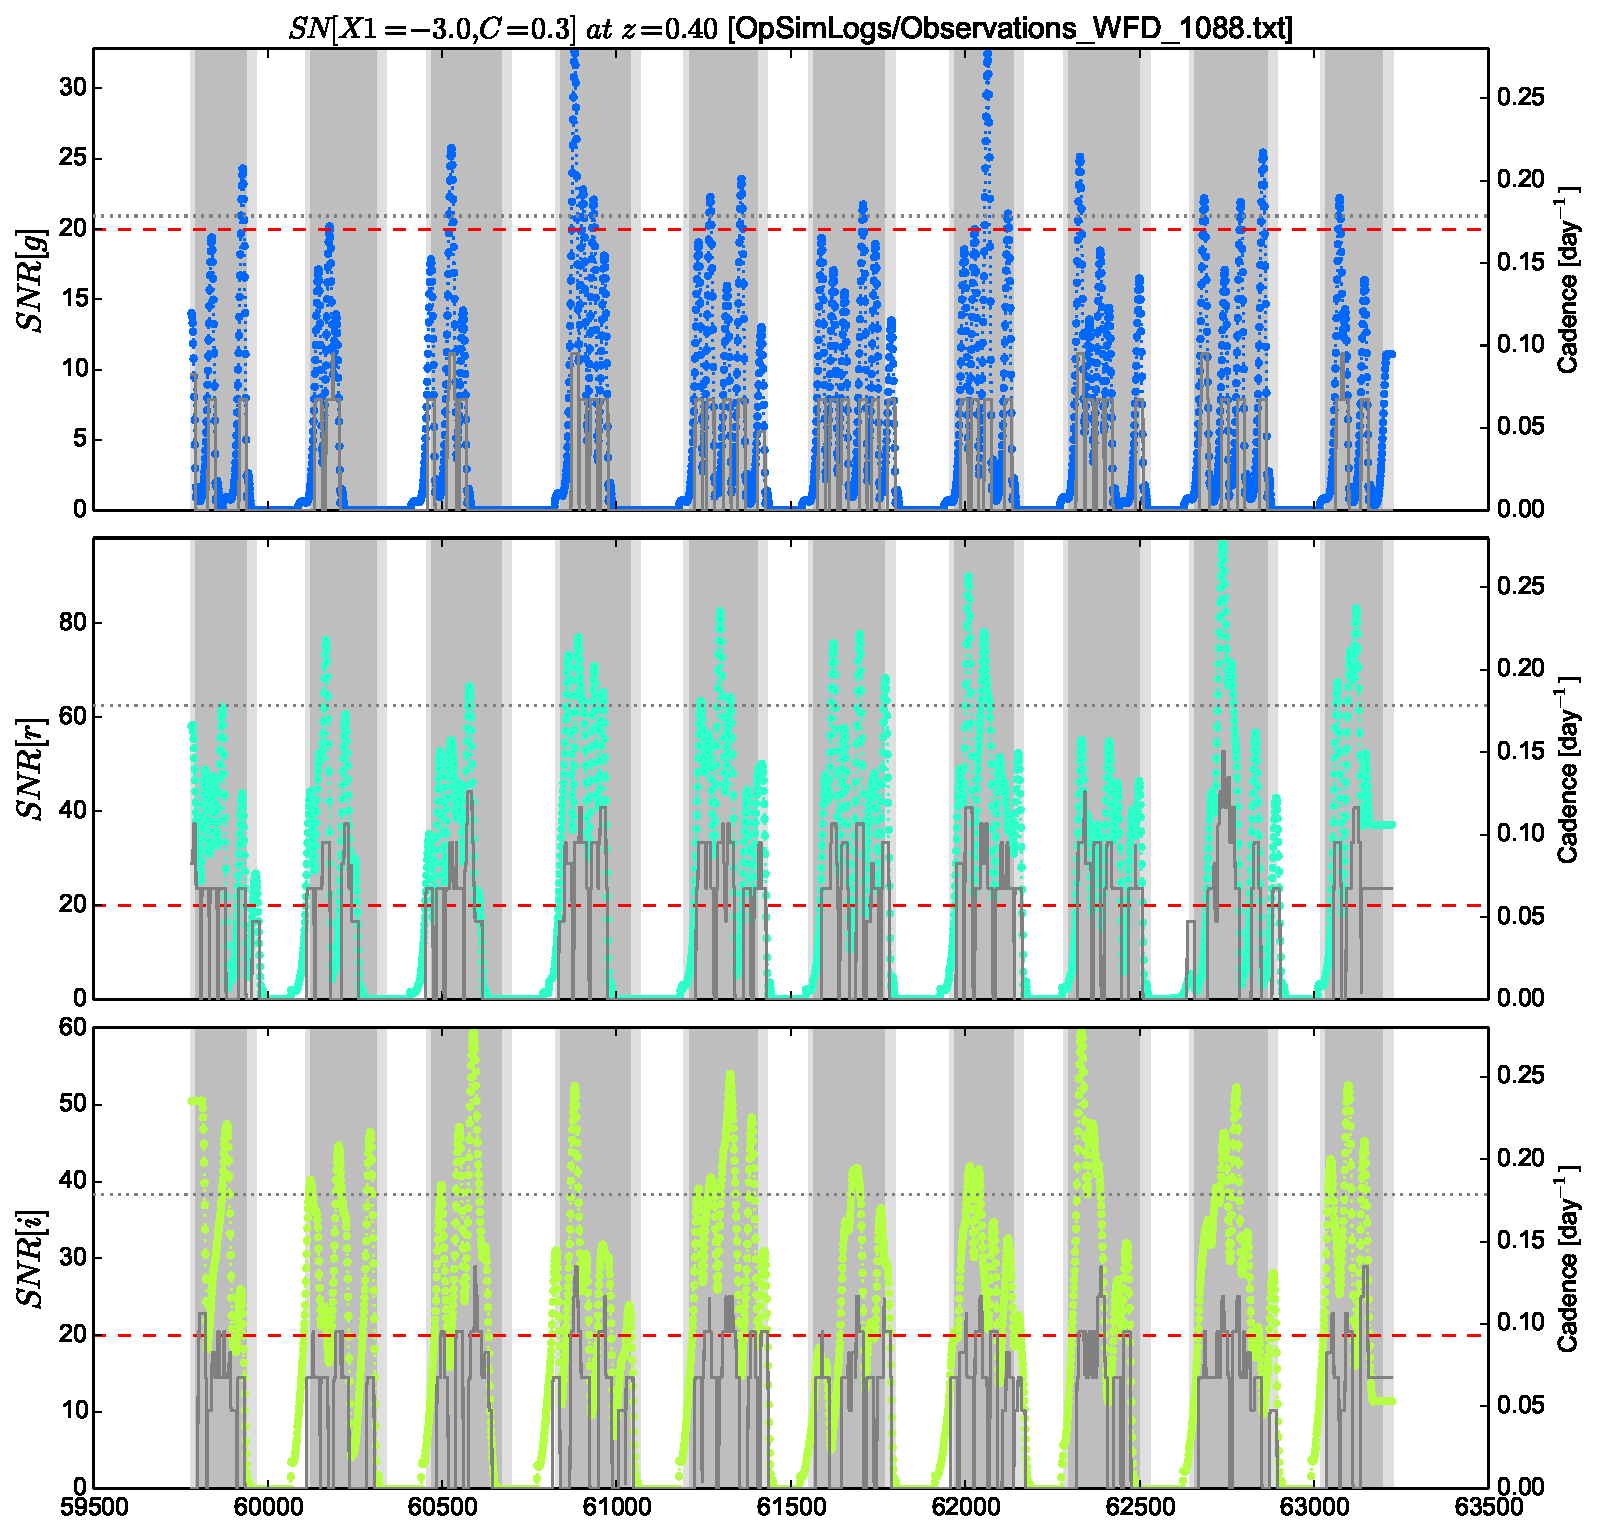
\includegraphics[width=\linewidth]{metric_WFD_1088.pdf}
    \caption{}
  \end{center}
\end{figure*}




\end{document}
% ======================================================================
% 








% There are a number of useful \LaTeX\xspace commands predefined in
% \code{macros.tex}.  Notice that the section labels are prefixed with
% \code{sec:} to allow the use of the \verb=\secref= command to
% reference a section (\ie, \secref{intro}).  Figures can be referenced
% with the \verb=\figref= command, which assumes that the figure label
% is prefixed with \code{fig:}.  In \figref{example} we show an example
% figure.  You'll notice that the actual figure file is found in the
% \code{figures} directory.  However, because we have specified this
% directory in our \verb=\graphicspath= we do not need to explicitly
% specify the path to the image.

% The \code{macros.tex} package also contains some conventional
% scientific units like \angstrom, \GeV, \Msun, etc. and some editorial
% tools for highlighting \FIXME{issues}, \CHECK{text to be checked},
% \COMMENT{comments}, and \NEW{new additions}.
